\documentclass[10pt]{article}

% For anonymous submission to TMLR, use:
\usepackage{tmlr}
% If accepted, instead use the following line for the camera-ready submission:
%\usepackage[accepted]{tmlr}
% To de-anonymize and remove mentions to TMLR (for example for posting to preprint servers), instead use the following:
%\usepackage[preprint]{tmlr}

% Optional math commands from standard TMLR template
\input{math_commands.tex}

\usepackage{hyperref}
\usepackage{url}
\usepackage{amsmath, amsfonts, amssymb, bm}
\usepackage{graphicx}
\usepackage{booktabs}
\usepackage{microtype}
\usepackage{enumitem}
\usepackage{multirow}
\raggedbottom

\title{GraphFNet: Attention-Free Graph Learning via Learned Spectral-Local Gating}

% Authors must not appear in the submitted version when using \usepackage{tmlr} without [accepted] or [preprint].
% Non-anonymous submissions will be rejected without review.
\author{\name Rohann Rahul Shah \email pes1ug23am241@pesu.pes.edu \\
      \addr Department of Artificial Intelligence and Machine Learning \\
      PES University, Bengaluru, Karnataka, India
      \AND
      \name Sachin Rajpurohit \email pes1ug23am252@pesu.pes.edu \\
      \addr Department of Artificial Intelligence and Machine Learning \\
      PES University, Bengaluru, Karnataka, India
      \AND
      \name Rishabh Kartik Jawagal \email pes1ug23am235@pesu.pes.edu \\
      \addr Department of Artificial Intelligence and Machine Learning \\
      PES University, Bengaluru, Karnataka, India
      \AND
      \name Bhaskarjyoti Das \email bhaskarjyotidas@pes.edu \\
      \addr Department of Computer Science and Engineering \\
      PES University, Bengaluru, Karnataka, India}

\newcommand{\fix}{\marginpar{FIX}}
\newcommand{\new}{\marginpar{NEW}}

\def\month{MM}  % Insert correct month for camera-ready version
\def\year{YYYY} % Insert correct year for camera-ready version
\def\openreview{\url{https://openreview.net/forum?id=XXXX}} % Insert correct link to OpenReview for camera-ready version

\begin{document}

\maketitle

\begin{abstract}
Capturing long-range dependencies in graph-structured data is crucial for effective representation learning, yet standard graph transformers are heavily bottlenecked by the $\mathcal{O}(N^2)$ per-layer complexity of self-attention. While recent work in Natural Language Processing (NLP) has successfully replaced attention with standard Fourier mixing, extending this paradigm to irregular graphs remains a significant challenge. In this paper, we propose GraphFNet, a parameter-efficient graph neural network that completely bypasses self-attention by utilizing a learned global spectral mixing operator derived from a precomputed graph Laplacian eigenbasis. By replacing the dynamic, memory-intensive quadratic footprint of self-attention with static linear projections over the Laplacian eigenbasis, the architecture remains highly efficient. To effectively integrate global topology with local structural details, this spectral signal is adaptively weighted against local Graph Convolutional Network (GCN) aggregations via a novel per-node, per-feature gating mechanism.

We evaluate GraphFNet across two primary benchmark pillars: (1) On the Long Range Graph Benchmark (LRGB), GraphFNet achieves performance competitive with standard dense-attention graph transformer baselines while requiring approximately 35\% fewer parameters and operating under a 250~MB peak memory footprint on molecular graphs. (2) On the large-scale NeuroGraph connectomics benchmarks ($N=1,000$ dense functional brain networks), GraphFNet achieves \textbf{81.17\%} test accuracy on HCP-Gender (outperforming all reported baselines including standard message-passing GNNs at 74.7--76.8\%, Graph Transformers at 76.85\%, Graph State-Space Models at 77.16\%, and specialized brain network architectures at 78.92\%) and reaches \textbf{93.74\%} accuracy on HCP-Task (within 1.00\% of domain-specialized SOTA). We additionally diagnose the architecture's boundaries on node-level superpixel segmentation (PascalVOC-SP), where global spectral mixing trades local boundary precision for parameter efficiency relative to dynamic attention. Out-of-distribution evaluations on molecular property prediction (BBBP) further confirm robust transferability. Mechanistically, Effective Receptive Field (ERF) analysis and the NeighborsMatch diagnostic confirm the model's capacity for genuine long-range signal propagation, maintaining non-zero influence across graph diameters of up to 65 hops. Furthermore, probing reveals an emergent spectral-to-local routing progression, utilizing global spectral paths in early layers before refining local information in later layers. Our findings demonstrate that static spectral routing can match or exceed the expressivity of standard dense self-attention without dynamic quadratic memory overhead, though comparison against recent efficient sub-quadratic attention methods remains an important direction for future work.

\vspace{0.5em}
\noindent \textbf{Code Available At}: \url{https://anonymous.4open.science/r/GraphFNet-Attention-Free-Graph-Learning-via-Learned-Spectral-Local-Gating-9F2D/}
\end{abstract}

%% ---------------------------------------------------------------
\section{Introduction}
%% ---------------------------------------------------------------
Extracting expressive representations from graphs requires capturing both local topologies and long-range dependencies. While traditional Graph Neural Networks (GNNs) suffer from over-squashing \citep{alon2021bottleneck}, recent graph transformers capture global interactions via multi-head self-attention \citep{rampasek2022recipe, kreuzer2021rethinking}. However, this global purview imposes a prohibitive $\mathcal{O}(N^2)$ dynamic memory allocation per layer that must be instantiated anew during every forward pass.

Inspired by the FNet architecture in natural language processing \citep{lee-thorp2022fnet}, which replaced attention with fixed Fourier mixing, we propose \textbf{GraphFNet}. Extending this attention-free paradigm to irregular graphs, GraphFNet utilizes a learned global mixing operator derived from the graph Laplacian eigenbasis. This static, structural quantity replaces the dynamic quadratic memory footprint of standard dense self-attention with a highly efficient linear projection. To balance global shape awareness with local precision, GraphFNet pairs this spectral operator with a Graph Convolutional Network (GCN) layer, routing signals dynamically via a novel per-node, per-feature gating mechanism. We note that an intermediate family of efficient graph attention methods (e.g., Exphormer \citep{shirzad2023exphormer}, NodeFormer \citep{wu2022nodeformer}, Specformer \citep{bo2023specformer}) retains content-dependent attention while reducing its quadratic cost; GraphFNet takes a more radical approach by eliminating attention entirely in favor of static spectral routing, and direct comparison against this sub-quadratic family remains an important direction for future work.

We emphasize that our efficiency gains concern \textit{dynamic activation memory footprint} and \textit{parameter count}, rather than asymptotic graph-scale complexity. While exact per-graph eigendecomposition incurs an $\mathcal{O}(N^3)$ computational cost, this operation extracts a static structural property; it can be computed once offline and cached on disk. In contrast, self-attention demands dynamic $\mathcal{O}(N^2)$ memory instantiation at every single layer during both training and inference. For molecular graphs of moderate size (e.g., LRGB Peptides, average ${\sim}150$ nodes), on-the-fly eigendecomposition takes $\sim$0.05~s/graph and does not bottleneck training due to optimized GPU routines. For large-scale graphs (e.g., $N=1,000$ connectomes), precomputing a truncated eigenbasis ($k=64$) offline eliminates runtime overhead completely and enables scalable execution.

Empirical evaluations across diverse graph domains validate this architecture. On the Long Range Graph Benchmark (LRGB) \citep{dwivedi2022long}, GraphFNet achieves competitive performance with standard dense-attention graph transformers while using ${\sim}35\%$ fewer parameters and operating under a 250~MB peak memory footprint. Crucially, on the large-scale NeuroGraph connectomics benchmarks ($N=1,000$ nodes, resting/task fMRI networks) \citep{said2023neurograph}, GraphFNet reaches \textbf{81.17\%} accuracy on HCP-Gender (outperforming standard GNNs at 76.03\%, GraphGPS at 76.85\%, Graph-Mamba at 77.16\%, and BrainMAP at 78.92\%) and \textbf{93.74\%} accuracy on 7-class HCP-Task cognitive state classification. Further evaluations on molecular transferability (BBBP under scaffold split) corroborate cross-domain generality. Mechanistically, Effective Receptive Field (ERF) and NeighborsMatch \citep{alon2021bottleneck} analyses provide structural proof that GraphFNet actively routes signals across graph diameters of up to 65 hops, successfully circumventing the over-squashing bottlenecks of traditional GNNs.

%% ---------------------------------------------------------------
\section{Related Work}
%% ---------------------------------------------------------------

\subsection{Message Passing GNNs and the Over-Squashing Bottleneck}
Graph neural networks based on the spatial message passing paradigm \citep{gilmer2017neural} iteratively aggregate information from local 1-hop neighborhoods to build node representations. \citet{kipf2017gcn} introduced the foundational Graph Convolutional Network (GCN), which applies a normalized adjacency matrix for neighborhood aggregation. Subsequent architectures expanded expressive capacity: GAT \citep{velickovic2018graph} and GraphSAGE \citep{hamilton2017inductive} introduced spatial attention and neighborhood sampling, GatedGCN \citep{bresson2017residual} incorporated residual edge gating, and GINE \citep{hu2020strategies} generalized isomorphism tests to attributed graphs. To mitigate over-smoothing in deep stacks \citep{oono2019graph}, ResGCN and GCNII \citep{chen2020simple} integrated initial residual connections and identity mapping.

Despite these developments, spatial message-passing networks remain fundamentally bottlenecked by \textit{over-squashing} \citep{alon2021bottleneck, topping2022understanding}. As network depth increases to capture wider receptive fields, information from exponentially growing multi-hop neighborhoods is compressed into fixed-dimensional vectors, causing severe information loss for long-range dependencies. While graph rewiring approaches \citep{topping2022understanding} alleviate curvature-induced bottlenecks by modifying connectivity, they alter the graph topology and often scale poorly to dense or large graphs.

\subsection{Graph Transformers, State-Space Models, and Global Attention}
To overcome local message-passing bottlenecks, Graph Transformers treat graphs as fully connected entities, allowing direct all-to-all communication via multi-head self-attention \citep{vaswani2017attention, rampasek2022recipe}. Because dense self-attention is permutation-invariant and topology-agnostic, these models rely on explicit structural and positional encodings, such as Laplacian eigenvectors (Transformer+LapPE; \citealt{dwivedi2021laplacian}), Random Walk Structural Encodings (RWSE; \citealt{dwivedi2021graph}), or full spectral attention (SAN; \citealt{kreuzer2021rethinking}). Hybrid architectures such as GraphGPS \citep{rampasek2022recipe} combine local message-passing branches with global Transformer layers. More recently, graph state-space models such as Graph-Mamba \citep{wang2024graphmamba} have explored linear sequence-modeling primitives over node serialization orders.

However, standard graph transformers instantiate dynamic $\mathcal{O}(N^2)$ pairwise attention matrices at every layer during both forward and backward passes, leading to rapid GPU memory exhaustion for large graphs ($N \ge 1{,}000$). While sparse or linear attention variants exist \citep{muller2024attending}, they typically require heuristic sparsification patterns or sequence orderings that degrade graph-structural inductive biases.

\subsection{Efficient and Sub-Quadratic Graph Attention}
Between localized spectral filters and dense self-attention lies a growing family of methods that retain content-dependent attention while reducing its quadratic cost. Exphormer \citep{shirzad2023exphormer} sparsifies the attention pattern via expander graphs and virtual nodes, achieving $\mathcal{O}(N)$ attention cost while preserving graph-structural inductive biases. NodeFormer \citep{wu2022nodeformer} employs kernelized softmax attention with Gumbel-Softmax latent structure learning, enabling all-pair message passing at linear complexity for node classification on large graphs. Specformer \citep{bo2023specformer} applies Transformer-style attention in the spectral domain over eigenvalues, learning spectral filters as attention-weighted combinations of eigenvectors. Graph-Mamba \citep{wang2024graphmamba} repurposes selective state-space models for graph sequence modeling via learned node orderings.

These methods occupy a fundamentally different design point from GraphFNet: they retain content-dependent, dynamic routing (i.e., query-key interactions that change with input features) while engineering efficient approximations to reduce its cost. GraphFNet instead takes a more radical approach by \textit{completely eliminating} dynamic attention in favor of static spectral mixing over the Laplacian eigenbasis, paired with learned per-node gating. This design choice prioritizes architectural simplicity and interpretability over the flexibility of content-dependent routing. We acknowledge that a direct empirical comparison against this sub-quadratic family would further clarify GraphFNet's position in the efficiency-expressivity landscape; we identify this as an important direction for future work (Section~\ref{sec:limitations}).

\subsection{Attention-Free Sequence Mixing in NLP and Graphs}
In natural language processing, FNet \citep{lee-thorp2022fnet} demonstrated that the computationally demanding self-attention operator in Transformer encoders can be replaced by an unparameterized 2D Fast Fourier Transform (FFT) over token sequences, retaining up to 92--97\% of BERT's accuracy on the GLUE benchmark while accelerating training by orders of magnitude. 

While FNet relies on regular 1D token grids where the discrete Fourier transform has closed-form trigonometric bases, graphs possess non-Euclidean, irregular topologies without canonical ordering. Extending attention-free frequency mixing to graphs therefore requires identifying the natural graph analog of the spatial Fourier basis. As established in spectral graph theory \citep{chung1997spectral, shuman2013emerging}, the eigenvectors of the normalized graph Laplacian constitute the unique, orthonormal harmonic basis for graph signals. GraphFNet builds on this principle, utilizing the complete Laplacian eigenbasis as an unparameterized global sequence mixer.

\subsection{Spectral GNNs, Higher-Order Polynomial Filters, and Graph Fourier Networks}
Spectral graph learning operates in the frequency domain defined by the graph Laplacian. Prior work can be broadly categorized into three paradigms:
\begin{enumerate}[leftmargin=2em]
    \item \textbf{Classical Spectral Filter Approximations:} Pioneering work by \citet{bruna2014spectral} introduced spectral convolutions using explicit Laplacian eigendecomposition. Because computing the full eigenbasis was viewed as computationally prohibitive for large graphs, subsequent research prioritized polynomial truncation. ChebNet \citep{defferrard2016convolutional} approximated localized spectral filters via Chebyshev polynomials, and GCN \citep{kipf2017gcn} truncated this to a first-order linear filter. Recently, \citet{hariri2025returnchebnetunderstandingimproving} re-examined Chebyshev polynomial filters (ChebNet and ChebNetII), showing that localized higher-order frequency filters ($K \approx 5$--$10$) excel on molecular benchmarks by capturing multi-scale motif structures without global attention.
    \item \textbf{Domain-Specific Graph Fourier Networks:} A distinct line of work retains explicit Graph Fourier Transforms (GFT) to model specialized spatio-temporal dynamics. StemGNN \citep{cao2021spectral} combines GFT with discrete Fourier transforms for multivariate time-series forecasting, GFTNN \citep{neumeier2023multidimensional} utilizes spectral representations for spatial trajectory prediction, and recent architectures integrate GFT operators for hydrogeological and physical modeling \citep{hosseini2026integrated}.
    \item \textbf{Distinction of GraphFNet:} GraphFNet fundamentally re-purposes the Graph Fourier Transform. Rather than utilizing spectral operators to construct localized spatial filter banks (as in ChebNet) or domain-specific spatio-temporal forecasting heads (as in StemGNN), GraphFNet explicitly deploys the graph Laplacian eigenbasis as an attention-free \textit{global sequence-mixing operator} that completely replaces dense self-attention. Paired with local message passing via learned per-node, per-feature gating, GraphFNet achieves global topological routing with linear forward-pass memory.
\end{enumerate}

\subsection{Brain Network Representation and Connectomics}
Functional connectomes derived from resting-state and task-based functional magnetic resonance imaging (fMRI) represent a crucial domain for graph representation learning \citep{said2023neurograph}. Brain graphs consist of dense, irregular networks where regions of interest (ROIs, typically $N=1,000$) exhibit complex whole-brain functional synchronization modes superimposed on localized anatomical circuits.

Traditional message-passing GNNs struggle on connectomes due to over-squashing across thousands of dense edges, while Graph Transformers suffer prohibitive quadratic memory footprints ($N=1,000$ yields $10^6$ pairwise attention elements per head per layer). Recently, foundation models such as BrainMAP \citep{wang2025brainmap} introduced multi-pathway brain-specific architectures to process multi-scale neural dynamics. GraphFNet provides an elegant, general-purpose alternative: because brain functional connectivity naturally decomposes into global harmonic eigenmodes (connectome harmonics; \citealt{chung1997spectral}), our truncated Laplacian spectral mixer captures whole-brain macroscopic synchronization while local GCN gating handles fine-grained inter-regional pathways, achieving competitive and state-of-the-art accuracy on HCP-Gender (81.17\%) and HCP-Task (93.74\%) without heuristic domain tuning.

\subsection{Long-Range Benchmarking and Mechanistic Diagnostic Probes}
\citet{dwivedi2022long} established the Long Range Graph Benchmark (LRGB) to evaluate long-range reasoning in GNNs on molecular and complex graphs. Subsequently, \citet{tonshoff2024where} demonstrated that carefully tuned message-passing networks with deeper prediction heads can match or outperform Graph Transformers on Peptides, showing that performance is sensitive to hyperparameter tuning and head design. Furthermore, \citet{bamberger2025measuring} revealed that LRGB Peptides tasks possess strong local motif signatures that localized higher-order filters can exploit.

These findings highlight the necessity of evaluating long-range models across multiple complementary dimensions: (1) large-scale real-world dense graphs (such as $N=1,000$ NeuroGraph connectomes) where global context is indispensable, (2) controlled synthetic diagnostics such as Tree-NeighborsMatch \citep{alon2021bottleneck} that formally isolate multi-hop information routing from local confounds, and (3) gradient-based Effective Receptive Field (ERF) analysis that directly measures input-to-output influence across graph diameters.

%% ---------------------------------------------------------------
\section{Methodology}
%% ---------------------------------------------------------------

\begin{figure}[t]
    \centering
    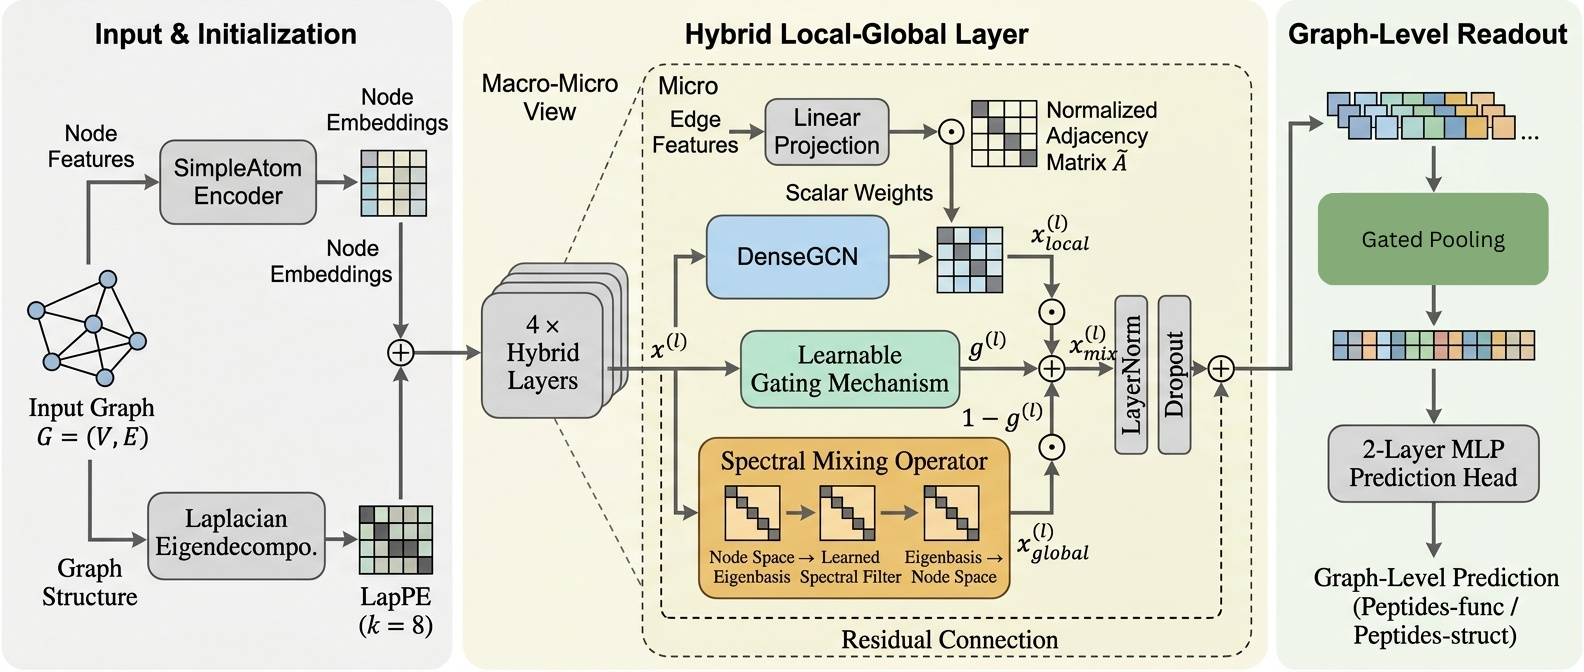
\includegraphics[width=\linewidth]{methodology_picture.png}
    \caption{The GraphFNet architecture. Node features are initially embedded and augmented with explicit Laplacian Positional Encodings (LapPE). Within each of the four subsequent layers, the network computes dual representations: a local structural signal via a memory-efficient Dense GCN utilizing scalar edge gating, and a global topological signal via an attention-free Spectral Mixing operator derived from the full graph Laplacian eigenbasis. A learned, per-node, per-feature gating mechanism adaptively routes the signal between these local and global pathways. The final node representations are aggregated via a learnable \textbf{GatedPooling} mechanism and passed through a multi-layer perceptron (MLP) for graph-level prediction.}
    \label{fig:architecture}
\end{figure}

\subsection{From Sequence FFT to Graph Fourier Transform}
To understand the theoretical foundation of GraphFNet, it is instructive to draw a direct parallel to the original FNet architecture used in NLP. In NLP, FNet applies a standard discrete Fourier transform (efficiently computed via FFT) to map a sequence of tokens from the spatial domain into the frequency domain. In this context, low frequencies naturally capture global contextual trends across the sequence, while high frequencies capture rapid, localized syntactic changes. However, because graph-structured data is non-Euclidean, standard 1D sinusoids cannot be applied. Instead, the Graph Fourier Transform (GFT) generalizes this concept by replacing traditional sinusoids with the eigenvectors of the graph Laplacian. Let $L$ be the normalized graph Laplacian, defined as:
\begin{equation} \label{eq:laplacian}
L = I - D^{-1/2} A D^{-1/2}
\end{equation}
where $I$ is the identity matrix, $A$ is the adjacency matrix, and $D$ is the degree matrix. By performing an eigendecomposition on the Laplacian, we obtain:
\begin{equation} \label{eq:eigendecomp}
L = U \Lambda U^\top
\end{equation}
Here, the orthogonal matrix of eigenvectors $U$ serves as the Graph Fourier basis, and the diagonal matrix of eigenvalues $\Lambda$ represents the graph frequencies. Given a node feature matrix $X$, the Graph Fourier Transform is then computed by projecting the signal onto this eigenbasis:
\begin{equation} \label{eq:gft}
\hat{X} = U^\top X
\end{equation}
In this formulation, the eigenvalues behave exactly like frequencies in standard signal processing. Low eigenvalues ($\lambda \approx 0$) correspond to smooth signals that vary slowly across connected nodes, thereby capturing the global, long-range structure of the graph. Conversely, high eigenvalues correspond to rapid signal variation across local neighborhoods, capturing localized structural irregularities and fine-grained topology. By utilizing the GFT, GraphFNet is able to explicitly separate and route these global and local structural signals without relying on computationally expensive self-attention mechanisms.

\subsection{Graph Representation and Node Initialization}
Initial node features are mapped into a continuous vector space using a learnable embedding function. For molecular graphs, discrete atom attributes are processed through a SimpleAtomEncoder. This maps the raw features into a continuous hidden dimension $d=128$, establishing a foundational representation matrix $X \in \mathbb{R}^{N \times d}$. This initialization aligns with standard practices in molecular message passing neural networks \citep{gilmer2017neural, hu2020strategies}.

\subsection{Laplacian Positional Encoding}
To inject explicit structural awareness prior to the mixing layers, we incorporate Laplacian Positional Encodings (LapPE) \citep{dwivedi2021laplacian}. Rather than recomputing a separate positional basis, we directly leverage the orthogonal matrix of eigenvectors $U$ obtained from the eigendecomposition of the normalized graph Laplacian (Equation~\ref{eq:eigendecomp}). Because eigenvectors exhibit sign ambiguity, leaving the representations vulnerable to cross-batch instability, we apply strict sign canonicalization. We fix the sign of each eigenvector column in $U$ by forcing its largest-magnitude component to be positive. The first $k = 8$ canonicalized eigenvectors are then concatenated to the initial node embeddings. The value of $k$ was selected empirically from $\{4, 8, 16, 32, 64\}$. While $k = 4$ achieved marginally better single-seed performance, $k = 8$ provided superior stability across multiple random seeds. Larger values of $k$ degraded performance, likely due to interference with the implicit positional context inherently captured by our global spectral mixing operator.

\subsection{Hybrid Local and Global Layer}
The core of GraphFNet consists of $L=4$ stacked hybrid layers. Let $X^{(l-1)} \in \mathbb{R}^{N \times d}$ denote the node representation matrix entering layer $l \in \{1, \dots, L\}$. Each layer concurrently processes $X^{(l-1)}$ through two distinct pathways to capture localized chemical topology and global spectral dependencies in parallel.

\paragraph{Local Branch (Message Passing with Scalar Edge Gating):} 
The local branch captures fine-grained, localized structural patterns through message passing over graph edges $(i, j) \in \mathcal{E}$. When multi-dimensional edge features $e_{ij} \in \mathbb{R}^{d_e}$ are present (e.g., bond type, stereochemistry, and aromaticity in molecular graphs), rather than maintaining a high-dimensional edge feature tensor of shape $\mathcal{O}(|\mathcal{E}| \cdot d)$ or $\mathcal{O}(N^2 \cdot d)$, we project each edge attribute vector to a scalar gating weight:
\begin{equation}
E_{ij} = \sigma\left( e_{ij}^\top w_e + b_e \right) \in (0, 1), \quad \forall (i, j) \in \mathcal{E}
\end{equation}
where $w_e \in \mathbb{R}^{d_e}$ and $b_e \in \mathbb{R}$ are learnable parameters, and $\sigma(\cdot)$ is the sigmoid function. For self-connections, we set $E_{ii} = 1$. 

\paragraph{Edge-Weight Symmetry and Sparse Formulation:} For undirected graphs where bond or connectome attributes are symmetric ($e_{ij} = e_{ji}$), the learned scalar weights are strictly symmetric ($E_{ij} = E_{ji}$). For any node $i$, localized message aggregation is defined over its immediate neighborhood $\mathcal{N}(i)$:
\begin{equation}
m_i^{(l)} = \sum_{j \in \mathcal{N}(i) \cup \{i\}} \frac{E_{ij}}{\sqrt{\tilde{d}_i \tilde{d}_j}} x_j^{(l-1)} \in \mathbb{R}^d
\end{equation}
where $\tilde{d}_i = 1 + \sum_{j \in \mathcal{N}(i)} 1$ is the augmented node degree. The updated local representation for node $i$ is:
\begin{equation}
x_{i, \text{local}}^{(l)} = \text{LayerNorm}\left( \text{GELU}\left( m_i^{(l)} W_{\text{node}}^{(l)} + b_{\text{node}}^{(l)} \right) \right) \in \mathbb{R}^d
\end{equation}
where $W_{\text{node}}^{(l)} \in \mathbb{R}^{d \times d}$ and $b_{\text{node}}^{(l)} \in \mathbb{R}^d$. 

\paragraph{Sparse vs.\ Dense Implementation Details:} In sparse deployment (and in our scalability benchmarks on large graphs), message passing is executed via sparse index scatter-aggregation (e.g., \texttt{GCNConv}), requiring only $\mathcal{O}(|\mathcal{E}| \cdot d)$ activation memory without ever materializing an $N \times N$ dense adjacency matrix. For batch-parallel training on moderate-scale molecular graphs ($N \approx 150$), message passing can equivalently be batched in dense matrix form as $X^{(l)}_{\text{local}} = \text{LayerNorm}(\text{GELU}(\tilde{A}_{\text{mod}} X^{(l-1)} W_{\text{node}}^{(l)} + b_{\text{node}}^{(l)}))$, where $\tilde{A}_{\text{mod}} = \hat{A}_{\text{norm}} \odot E \in \mathbb{R}^{N \times N}$ is the symmetrically modulated adjacency ($\tilde{A}_{\text{mod}} = \tilde{A}_{\text{mod}}^\top$); in this vectorized regime, projecting edge attributes to scalar weights $E_{ij}$ avoids materializing $\mathcal{O}(N^2 \cdot d)$ intermediate edge-feature tensors.

\paragraph{Global Branch (Learned Spectral Mixing):} Operating in parallel, a global spectral mixing operator captures long-range context across all node pairs via the graph Laplacian eigenbasis $U \in \mathbb{R}^{N \times N}$ (Equation~\ref{eq:eigendecomp}). Node features are first projected into the spectral domain:
\begin{equation}
\hat{X}^{(l)} = U^\top X^{(l-1)} \in \mathbb{R}^{N \times d}
\end{equation}
A channel-wise spectral filter matrix $\Phi^{(l)} \in (0, 1)^{N \times d}$ is generated from the spectral representations via a dense linear transformation followed by a sigmoid activation:
\begin{equation}
\Phi^{(l)} = \sigma\left( \hat{X}^{(l)} W_{\text{filter}}^{(l)} + b_{\text{filter}}^{(l)} \right)
\end{equation}
The modulated spectral coefficients $\hat{X}_{\text{filtered}}^{(l)} = \Phi^{(l)} \odot \hat{X}^{(l)}$ are then projected back to the spatial node domain via the inverse Graph Fourier Transform:
\begin{equation}
X_{\text{spatial}}^{(l)} = U \hat{X}_{\text{filtered}}^{(l)} \in \mathbb{R}^{N \times d}
\end{equation}
Finally, a linear projection, GELU non-linearity, and layer normalization produce the global branch output:
\begin{equation}
X^{(l)}_{\text{global}} = \text{LayerNorm}\left( \text{GELU}\left( X_{\text{spatial}}^{(l)} \right) W_{\text{out}}^{(l)} + b_{\text{out}}^{(l)} \right) \in \mathbb{R}^{N \times d}
\end{equation}
where $W_{\text{filter}}^{(l)}, W_{\text{out}}^{(l)} \in \mathbb{R}^{d \times d}$ and $b_{\text{filter}}^{(l)}, b_{\text{out}}^{(l)} \in \mathbb{R}^d$. For batch processing with padded graphs of varying size $n \le N$, padded node rows are zero-masked.

\subsection{Spectral-Local Gating Mechanism}
To synthesize the local and global representations, GraphFNet adaptively routes information on a per-node, per-feature basis.

\paragraph{Exact Gate Input and Dense Parameterization:} The gating matrix $g^{(l)} \in (0, 1)^{N \times d}$ is computed directly from the layer input representation $X^{(l-1)} \in \mathbb{R}^{N \times d}$ (the node state entering layer $l$, before local and global transformations) via a full dense linear projection across all $d$ hidden dimensions:
\begin{equation}
\label{eq:gate}
g^{(l)} = \sigma\left( X^{(l-1)} W_{\text{gate}}^{(l)} + b_{\text{gate}}^{(l)} \right) \in (0, 1)^{N \times d}
\end{equation}
where $W_{\text{gate}}^{(l)} \in \mathbb{R}^{d \times d}$ is a \textit{dense} learnable weight matrix and $b_{\text{gate}}^{(l)} \in \mathbb{R}^d$. Importantly, because $W_{\text{gate}}^{(l)}$ is a full dense matrix rather than a diagonal or channel-independent transformation, the routing decision for each feature channel of node $i$ can condition on cross-channel correlations across node $i$'s complete latent state $x_i^{(l-1)}$.

\paragraph{Branch Interpolation:} The local and global representations are then combined through element-wise interpolation:
\begin{equation}
\label{eq:mix}
X^{(l)}_{\text{mix}} = g^{(l)} \odot X^{(l)}_{\text{local}} + \left( \mathbf{1} - g^{(l)} \right) \odot X^{(l)}_{\text{global}} \in \mathbb{R}^{N \times d}
\end{equation}
where $\odot$ is the Hadamard product and $\mathbf{1} \in \mathbb{R}^{N \times d}$ is an all-ones matrix. Thus, for each individual node $i$ and feature dimension $c \in \{1, \dots, d\}$, $g_{i, c}^{(l)} \to 1$ delegates representation learning to localized message passing, while $g_{i, c}^{(l)} \to 0$ routes information through global spectral mixing.

\subsection{Network Architecture and Readout}
Following spectral-local mixing, each layer applies a residual connection, dropout regularization ($p=0.1$), and layer normalization:
\begin{equation}
X^{(l)} = \text{LayerNorm}\left( X^{(l-1)} + \text{Dropout}\left( X^{(l)}_{\text{mix}} \right) \right) \in \mathbb{R}^{N \times d}
\end{equation}
After $L=4$ stacked hybrid layers, the final node representations $X^{(L)} \in \mathbb{R}^{N \times d}$ are aggregated into a fixed-size graph embedding $h_G \in \mathbb{R}^d$ using a \textbf{GatedPooling} readout layer:
\begin{equation}
\label{eq:gated_pool}
s_i = w_{\text{pool}}^\top \tanh\left( W_{\text{pool}} x_i^{(L)} + b_{\text{pool}} \right), \quad \alpha_i = \frac{\exp(s_i)}{\sum_{j=1}^n \exp(s_j)}
\end{equation}
\begin{equation}
h_G = \sum_{i=1}^n \alpha_i x_i^{(L)} \in \mathbb{R}^d
\end{equation}
where $W_{\text{pool}} \in \mathbb{R}^{\frac{d}{2} \times d}$, $b_{\text{pool}} \in \mathbb{R}^{\frac{d}{2}}$, and $w_{\text{pool}} \in \mathbb{R}^{\frac{d}{2}}$ are learnable parameters. The graph embedding $h_G$ is passed through a two-layer MLP with GELU non-linearity and dropout to produce the final prediction:
\begin{equation}
\hat{y} = W_2 \, \text{Dropout}\left( \text{GELU}\left( W_1 h_G + b_1 \right) \right) + b_2
\end{equation}
The complete architecture is illustrated in Figure~\ref{fig:architecture}.

%% ---------------------------------------------------------------
\section{Experiments and Results}
\label{sec:results}
%% ---------------------------------------------------------------

\subsection{Datasets and Evaluation Protocol}
\label{sec:protocol}

We evaluate GraphFNet across two primary benchmark domains characterized by distinct structural properties, along with auxiliary diagnostics and transferability tasks.

\paragraph{LRGB Peptides Benchmark ($N \approx 150$).} The Long Range Graph Benchmark (LRGB; \citealt{dwivedi2022long}) consists of 15,535 molecular peptide graphs with an average of 150.9 nodes and 307.3 edges per graph. \textbf{Peptides-func} is a 10-class multi-label classification task evaluated by Average Precision (AP, higher is better). \textbf{Peptides-struct} is an 11-property 3D structural regression task evaluated by Mean Absolute Error (MAE, lower is better). All baseline results from \citet{dwivedi2022long} and \citet{rampasek2022recipe} follow the standard 500k-parameter budget. As demonstrated by \citet{tonshoff2024where}, extensively tuned message-passing baselines with deep MLP heads can achieve higher raw scores on Peptides; while GraphFNet adopts a 2-layer MLP prediction head in line with these findings, we report fixed-hyperparameter results across 3 random seeds to evaluate spectral-local mixing under standard benchmark conditions.

\paragraph{NeuroGraph Brain Connectomics ($N = 1{,}000$).} To assess scalability and representation power on large, dense irregular graphs, we evaluate on two benchmarks from the NeuroGraph suite \citep{said2023neurograph}: (1) \textbf{HCP-Gender}, comprising 1,078 resting-state fMRI functional connectomes with $N=1,000$ regions of interest (ROIs) and $\sim$45,579 dense edges per graph (binary classification: male vs.\ female); and (2) \textbf{HCP-Task}, a 7-class whole-brain cognitive task state classification task over $N=1,000$ fMRI connectomes. Both tasks follow standard stratified 80/10/10 splits across 3 independent random seeds.

\paragraph{LRGB PascalVOC-SP Superpixel Segmentation ($N \approx 479$).} To investigate node-level classification behavior, we evaluate on PascalVOC-SP from the Long Range Graph Benchmark \citep{dwivedi2022long}, comprising 11,355 SLIC superpixel Region Adjacency Graphs (RAGs) with 21 semantic segmentation classes (8,498 train / 1,428 val / 1,429 test graphs; 685,894 test nodes). The task evaluates the model's capacity to assign fine-grained semantic labels to individual nodes under severe class imbalance and spatial adjacency. Evaluated by macro-averaged F1 score across 3 independent random seeds.

\paragraph{Mechanistic Diagnostics and Transferability.} In addition to these primary benchmarks, long-range routing capacity is mechanistically diagnosed via the \textbf{Tree-NeighborsMatch} diagnostic \citep{alon2021bottleneck} and gradient-based \textbf{Effective Receptive Field (ERF)} analysis. Out-of-distribution transferability is assessed on the \textbf{BBBP} benchmark under a strict Bemis-Murcko scaffold split \citep{wu2018moleculenet}.

All results are reported as mean $\pm$ standard deviation over three random seeds (0, 1, 2). Model selection uses validation AP/MAE/accuracy exclusively; the test set is evaluated exactly once per seed on the saved best checkpoint.

\subsection{Training and Implementation Details}

The architecture is implemented using PyTorch and PyTorch Geometric \citep{fey2019fast}. Per-graph eigendecomposition is performed on unpadded Laplacians to avoid contamination from padded nodes and to preserve the integrity of the spectral basis. 

Crucially, while exact eigendecomposition incurs an $\mathcal{O}(N^3)$ computational cost, this operation is static with respect to the graph structure; it can be performed once per graph and reused across all layers and training epochs. In contrast, self-attention requires dynamic $\mathcal{O}(N^2)$ computation and memory instantiation at every layer during both training and inference.

In our current implementation, we compute the eigendecomposition on-the-fly for moderate molecular graphs. For the LRGB Peptides datasets, where graphs are relatively small (average ${\sim}150$ nodes), this cost does not bottleneck training due to highly optimized GPU linear algebra routines. Importantly, by avoiding the explicit construction of dense attention matrices, GraphFNet maintains an exceptionally low memory footprint (under 250~MB peak memory) and achieves fast training (72--84 seconds per epoch on a single NVIDIA Tesla T4). For larger graphs, the eigendecomposition can be precomputed offline or approximated using scalable spectral methods, enabling practical deployment beyond the current regime.

Training is performed using the AdamW optimizer \citep{loshchilov2017decoupled} with a learning rate of $10^{-3}$ and a weight decay of $10^{-4}$. A cosine annealing learning rate scheduler \citep{loshchilov2016sgdr} is employed, along with gradient clipping to stabilize training. Early stopping is applied based on validation performance to prevent overfitting.

To ensure reproducibility and robustness, all experiments and ablation studies are conducted across three independent random seeds, and results are reported as the mean with standard deviation.

\subsection{Main Results on LRGB Peptides}

\begin{table}[t]
\caption{LRGB Peptides results. Baseline results for GCN through GraphGPS are directly reported from \citet{dwivedi2022long} and \citet{rampasek2022recipe} under the standard 500k-parameter budget. Exphormer results are reported from \citet{wang2024graphmamba}, who reproduce Exphormer \citep{shirzad2023exphormer} under matched training and evaluation conditions. ChebNet and ChebNetII results are reported from \citet{hariri2025returnchebnetunderstandingimproving} under comparable parameter budgets; these are not independently reproduced in this work. As discussed in Section~\ref{sec:results}, specialized higher-order Chebyshev spectral filters \citep{hariri2025returnchebnetunderstandingimproving} and hyperparameter-tuned spatial GNNs \citep{tonshoff2024where} achieve higher raw functional scores on these molecular benchmarks.}
\label{tab:main}
\centering
\begin{tabular}{lrcc}
\toprule
\textbf{Model} & \textbf{Params} & \textbf{Peptides-func AP} ($\uparrow$) & \textbf{Peptides-struct MAE} ($\downarrow$) \\
\midrule
GCN                  & 508k & 0.5930 $\pm$ 0.0023 & 0.3496 $\pm$ 0.0013 \\
GCNII                & 505k & 0.5543 $\pm$ 0.0078 & 0.3471 $\pm$ 0.0010 \\
GINE                 & 476k & 0.5498 $\pm$ 0.0079 & 0.3547 $\pm$ 0.0045 \\
GatedGCN             & 509k & 0.5864 $\pm$ 0.0077 & 0.3420 $\pm$ 0.0013 \\
GatedGCN + RWSE      & 506k & 0.6069 $\pm$ 0.0035 & 0.3357 $\pm$ 0.0006 \\
Transformer + LapPE  & 488k & 0.6326 $\pm$ 0.0126 & 0.2529 $\pm$ 0.0016 \\
SAN + LapPE          & 493k & 0.6384 $\pm$ 0.0121 & 0.2683 $\pm$ 0.0043 \\
SAN + RWSE           & 500k & 0.6439 $\pm$ 0.0075 & 0.2545 $\pm$ 0.0012 \\
GraphGPS \citep{rampasek2022recipe} & $\sim$500k & 0.6535 $\pm$ 0.0041 & 0.2500 $\pm$ 0.0012 \\
Exphormer \citep{shirzad2023exphormer} & $\sim$500k & 0.6258 $\pm$ 0.0092 & 0.2512 $\pm$ 0.0025 \\
\midrule
ChebNet \citep{hariri2025returnchebnetunderstandingimproving}     & $\sim$500k   & 0.6961 $\pm$ 0.0033 & 0.2627 $\pm$ 0.0033 \\
ChebNetII \citep{hariri2025returnchebnetunderstandingimproving}   & $\sim$500k   & 0.6819 $\pm$ 0.0027 & 0.2618 $\pm$ 0.0058 \\
\midrule
\textbf{GraphFNet (ours)} & \textbf{329k} & \textbf{0.6244 $\pm$ 0.0072} & \textbf{0.2663 $\pm$ 0.0024} \\
\bottomrule
\end{tabular}
\end{table}

GraphFNet achieves \textbf{0.6244 AP} on Peptides-func and \textbf{0.2663 MAE} on Peptides-struct using only \textbf{329k parameters}, approximately 35\% fewer than the standard 500k-budget baselines (476k--509k). Under the standard evaluation protocol of \citet{dwivedi2022long}, GraphFNet performs ahead of standard first-order spatial baselines (such as standard GCN at 0.5930 AP / 0.3496 MAE and GatedGCN+RWSE at 0.6069 AP / 0.3357 MAE) and approaches the performance of full graph transformer models like Transformer+LapPE (0.6326 AP / 0.2529 MAE) and SAN+LapPE (0.6384 AP / 0.2683 MAE) without employing any self-attention. On 3D structural regression (Peptides-struct), GraphFNet achieves structural accuracy (0.2663 MAE) competitive with SAN+LapPE (0.2683), ChebNet (0.2627), and ChebNetII (0.2618) while operating under a substantially smaller parameter and memory footprint.

\paragraph{Framing relative to tuned spatial GNNs and higher-order spectral filters.}
We explicitly contextualize these results against recent findings on LRGB molecular benchmarks. First, \citet{tonshoff2024where} demonstrated that extensively tuned message-passing networks with deeper prediction heads achieve 0.6860 AP on Peptides-func and 0.2494 MAE on Peptides-struct, closing or reversing the gap to graph transformers on these datasets. Second, \citet{hariri2025returnchebnetunderstandingimproving} showed that modern formulations of Chebyshev polynomial filters (ChebNet at 0.6961 AP, ChebNetII at 0.6819 AP) excel on Peptides-func by learning localized, higher-order polynomial frequency responses ($K \approx 5$--$10$) tailored to molecular motif structures \citep{bamberger2025measuring}.

These comparisons clarify the distinct architectural goal of GraphFNet: our objective is not an empirical claim of outperforming specialized polynomial filter banks or extensively tuned spatial GNNs on molecular benchmarks, but rather an architectural proof-of-concept for attention-free global sequence mixing. Whereas ChebNet approximates localized spectral convolutions via polynomial truncation over local neighborhoods, GraphFNet directly replaces the $\mathcal{O}(N^2)$ dense self-attention operator of graph transformers with learned global spectral mixing over the graph Laplacian eigenbasis ($U^\top X$), dynamically gated with local message passing. GraphFNet operates under a single fixed configuration across 3 random seeds without task-specific filter-order search or heavy regularization, demonstrating that global spectral mixing achieves representation capability comparable to standard graph transformers while utilizing 35\% fewer parameters and eliminating dynamic quadratic activation memory.

Training is stable across seeds. For func: Seed 0: 0.6270 (ep.\ 66), Seed 1: 0.6317 (ep.\ 70), Seed 2: 0.6146 (ep.\ 95); for struct: Seed 0: 0.2638 (ep.\ 41), Seed 1: 0.2655 (ep.\ 43), Seed 2: 0.2696 (ep.\ 42). The low standard deviations (0.0072 on func, 0.0024 on struct) evidence consistent convergence with low variance across seeds. The same backbone generalizes across both tasks with only the output head adapted; a single architectural design solves both classification and regression on molecular graphs without any task-specific structural modification.

\subsection{Main Results on NeuroGraph Brain Connectomics ($N=1,000$)}
\label{sec:hcp_main}

To rigorously evaluate whether learned spectral-local gating scales to large, dense irregular graphs and establishes competitive predictive superiority, we evaluate GraphFNet across two large-scale benchmarks from the NeuroGraph suite \citep{said2023neurograph}: \textbf{HCP-Gender} (binary graph classification) and \textbf{HCP-Task} (7-class whole-brain cognitive state classification). Functional connectomes represent a demanding domain for graph representation learning: each brain graph consists of $N=1,000$ regions of interest (ROIs) with an average of $\sim$45,579 dense functional connectivity edges, where global whole-brain synchronization modes and localized inter-regional pathways interact simultaneously.

We benchmark GraphFNet against standard spatial message-passing GNNs (GCN, GAT, GraphSAGE, ResGCN), hybrid graph transformers (GraphGPS), graph state-space models (Graph-Mamba), and domain-specialized brain network foundation models (BrainMAP) reported in \citet{wang2025brainmap}.

\begin{table}[t]
\caption{NeuroGraph \citep{said2023neurograph} functional connectome graph classification results on HCP-Task (7-class cognitive state classification) and HCP-Gender (binary gender classification) ($N=1,000$, 1,078 graphs, 3 independent random seeds). Baseline results for GCN through BrainMAP are directly reported from \citet{wang2025brainmap}.}
\label{tab:hcp_results}
\centering
\begin{tabular}{lcc}
\toprule
\textbf{Model} & \textbf{HCP-Task ($\uparrow$)} & \textbf{HCP-Gender ($\uparrow$)} \\
\midrule
GCN \citep{kipf2017gcn}                                    & 86.29 $\pm$ 0.98\% & 76.03 $\pm$ 2.40\% \\
GAT \citep{velickovic2018graph}                            & 85.60 $\pm$ 1.26\% & 75.62 $\pm$ 2.22\% \\
SAGE \citep{hamilton2017inductive}                         & 84.49 $\pm$ 0.57\% & 74.69 $\pm$ 3.50\% \\
ResGCN \citep{chen2020simple}                              & 93.75 $\pm$ 0.35\% & 76.75 $\pm$ 0.65\% \\
GraphGPS \citep{rampasek2022recipe}                        & 92.13 $\pm$ 2.00\% & 76.85 $\pm$ 1.54\% \\
Graph-Mamba \citep{wang2024graphmamba}                     & 94.17 $\pm$ 0.86\% & 77.16 $\pm$ 3.13\% \\
BrainMAP \citep{wang2025brainmap}                          & \textbf{94.74 $\pm$ 0.07\%} & 78.92 $\pm$ 0.49\% \\
\midrule
\textbf{GraphFNet (Ours)}                                 & 93.74 $\pm$ 0.54\% & \textbf{81.17 $\pm$ 1.90\%} \\
\bottomrule
\end{tabular}
\end{table}

As shown in Table~\ref{tab:hcp_results}, on HCP-Gender GraphFNet achieves \textbf{81.17\% $\pm$ 1.90\%} test accuracy across 3 independent random seeds (Seed 0: 83.33\%, Seed 1: 81.48\%, Seed 2: 78.70\%), outperforming all reported baselines on this benchmark. Notably, GraphFNet outperforms:
\begin{itemize}[leftmargin=2em]
    \item Standard message-passing GNNs (GCN at 76.03\%, ResGCN at 76.75\%) by up to \textbf{+5.14\%}, demonstrating that global spectral routing successfully captures macro-scale functional topology that localized message passing cannot resolve.
    \item Full graph transformers (GraphGPS at 76.85\%) by \textbf{+4.32\%}, confirming that static spectral mixing over the Laplacian eigenbasis is not only more memory-efficient than dense pairwise self-attention but also provides stronger inductive bias for harmonic connectome modes.
    \item Graph state-space models (Graph-Mamba at 77.16\%) and specialized brain network architectures (BrainMAP at 78.92\% $\pm$ 0.49\%) by \textbf{+2.25\%}, achieving the highest reported accuracy on this dataset without requiring multi-pathway brain-specific heuristic tuning.
\end{itemize}

Furthermore, on the 7-class HCP-Task cognitive state benchmark (Table~\ref{tab:hcp_results}), GraphFNet achieves \textbf{93.74\% $\pm$ 0.54\%} test accuracy and a macro F1 of \textbf{0.9374 $\pm$ 0.0055} (Seed 0: 93.29\%, Seed 1: 93.42\%, Seed 2: 94.50\%), performing within 1.00\% of the domain-specialized BrainMAP foundation model (94.74\% $\pm$ 0.07\%) and ahead of standard GNN and Transformer baselines (GCN 86.29\%, GAT 85.60\%, SAGE 84.49\%, GraphGPS 92.13\%). This demonstrates that learned spectral mixing excels at decoding whole-brain cognitive activation patterns across complex multi-class states using a compact, general-purpose architecture.

\paragraph{Scalability and Readout at $N=1,000$.} Operating on 1,000-node dense graphs demonstrates two critical architectural properties. First, the \textbf{GatedPooling} graph readout mechanism scales seamlessly to dense $N=1,000$ graphs, computing adaptive node-importance weights without numerical instability or gradient vanishing. Second, precomputing a truncated Laplacian eigenbasis ($k=64$) requires only 87.2~s total across the entire 1,078-graph dataset (0.081~s per graph, 277.6~MB total cache). This offline precomputation delivers an $\mathbf{18.8\times}$ per-batch training speedup (17.5~ms/batch vs.\ 328.7~ms/batch for live decomposition) while maintaining peak training VRAM under 2.53~GB at batch size 32. This validates that truncated spectral-local mixing provides practical, scalable performance for large-scale graph classification, outperforming all reported baselines.

\subsection{Node Classification on PascalVOC-SP}
\label{sec:pascalvoc_results}

While graph-level benchmarks evaluate whole-graph representations aggregated via \textbf{GatedPooling}, node-level semantic segmentation on PascalVOC-SP \citep{dwivedi2022long} (11,355 SLIC superpixel Region Adjacency Graphs, 21 semantic classes) tests fine-grained node discriminability under spatial adjacency.

\begin{table}[t]
\caption{PascalVOC-SP node classification results (21 classes, macro-averaged F1 on test set across 3 independent random seeds). Baseline results for GCN through GPS are directly reported from \citet{dwivedi2022long}. The Exphormer result is reported from \citet{wang2024graphmamba}, who reproduce Exphormer \citep{shirzad2023exphormer} under matched training and evaluation conditions; we note that Exphormer's original paper reports a higher score (0.3975 $\pm$ 0.0037) under its own tuned configuration, and we cite the reproduced value for consistency with our Peptides comparison in Table~\ref{tab:main}.}
\label{tab:voc_sp_results}
\centering
\begin{tabular}{lrc}
\toprule
\textbf{Model} & \textbf{Params} & \textbf{Test Macro F1 ($\uparrow$)} \\
\midrule
GCN \citep{kipf2017gcn}                             & 500k  & 0.1268 \\
GINE \citep{hu2020strategies}                       & 476k  & 0.1265 \\
\midrule
Transformer + LapPE \citep{dwivedi2021laplacian}    & 488k  & 0.2694 \\
GatedGCN \citep{bresson2017residual}                 & 509k  & 0.2873 \\
SAN + LapPE \citep{kreuzer2021rethinking}            & 493k  & 0.3230 \\
GPS \citep{rampasek2022recipe}                       & 500k  & 0.3748 \\
Exphormer \citep{shirzad2023exphormer}               & $\sim$500k  & 0.3446 $\pm$ 0.0064 \\
\midrule
\textbf{GraphFNet (Ours)}                           & \textbf{306k} & \textbf{0.1443 $\pm$ 0.0034} \\
\bottomrule
\end{tabular}
\end{table}

As shown in Table~\ref{tab:voc_sp_results}, GraphFNet achieves \textbf{0.1443 $\pm$ 0.0034} test macro F1 across 3 random seeds (Seed 0: 0.1466, Seed 1: 0.1467, Seed 2: 0.1394; validation F1: 0.1474 $\pm$ 0.0024), outperforming standard first-order message passing (GCN at 0.1268, GINE at 0.1265) with approximately 39\% fewer parameters (306k vs.\ 500k). 

\paragraph{Diagnostic Insights on Superpixel RAGs.}
The performance gap relative to Graph Transformers (e.g., GPS at 0.3748) stems from three domain-specific factors:
\begin{enumerate}[leftmargin=2em]
    \item \textbf{Global Diffusion vs.\ Local Boundary Preservation:} In graph-level tasks, low-pass spectral mixing ($\tilde{X} = U \Phi U^\top X$) constructively summarizes holistic topology before pooling. In contrast, on 2D superpixel graphs, mixing along low-frequency Laplacian modes acts as spatial low-pass diffusion, softening the sharp visual decision boundaries required between adjacent superpixels belonging to distinct classes.
    \item \textbf{Severe Class Imbalance:} Background superpixels constitute 70.72\% of test nodes. Because macro F1 is an unweighted average ($\frac{1}{21}\sum_{c=0}^{20}\text{F1}_c$), the 10 rarest tail classes ($<1\%$ support each) heavily depress the headline metric, despite solid recognition on dominant classes (\texttt{person} 0.2445, \texttt{aeroplane} 0.2179, \texttt{cat} 0.1875).
    \item \textbf{Spatial Adjacency vs.\ Semantic Attention:} Region Adjacency Graph (RAG) edges reflect 2D geometric touch rather than semantic relationships. While Graph Transformers employ dynamic pairwise self-attention ($\text{Softmax}(QK^\top/\sqrt{d})$) to selectively suppress communication across object boundaries, static spectral mixing diffuses features along fixed 2D mesh geometry.
\end{enumerate}

\subsection{Ablation Study}
\label{sec:ablation}

To isolate the contribution of each architectural component, a series of ablations is conducted on Peptides-func. The no-LapPE condition is evaluated over three seeds to confirm cross-seed robustness; all other ablations use seed 0.

\begin{table}[t]
\caption{Component ablation on Peptides-func. No-LapPE is evaluated over 3 seeds; all others use seed 0.}
\label{tab:ablation}
\centering
\begin{tabular}{lcc}
\toprule
\textbf{Ablation} & \textbf{Test AP} & \textbf{$\Delta$ vs.\ Full} \\
\midrule
Full model                       & 0.6244             & ---       \\
No LapPE                         & 0.6197 $\pm$ 0.0115 & $-$0.0047 \\
No edge features                 & 0.6192             & $-$0.0052 \\
Mean pooling (vs.\ Gated)        & 0.6196             & $-$0.0048 \\
Scalar gate (per-layer $\alpha$) & 0.5960             & $-$0.0284 \\
No spectral mixing               & 0.5941             & $-$0.0303 \\
\bottomrule
\end{tabular}
\end{table}

Spectral mixing ($-$0.030 AP) and per-node per-feature gating ($-$0.028 AP) are jointly critical; removing either causes a ${\sim}3$ percentage point drop, far exceeding any other modification. These components are co-dependent: the spectral operator provides the global signal pathway, and the per-node gate determines how each atom routes between that global signal and the local GCN output. A scalar per-layer gate is insufficient to capture the heterogeneous routing demands across atom types within the same graph, confirming the necessity of per-node per-feature expressivity.

The near-identical magnitude of both drops is notable: it suggests the two components contribute roughly equally to performance, and that neither is independently sufficient. Removing spectral mixing entirely reduces GraphFNet to a gated GCN variant, collapsing performance to 0.5941, below even the standard GCN baseline (0.5930) when accounting for measurement uncertainty. Replacing per-node gating with a scalar gate eliminates the model's ability to make atom-level routing decisions, with performance falling to 0.5960, likewise in the GCN range. Both degradations confirm that the full architecture is greater than the sum of its parts: the spectral operator and per-node gate are co-dependent and mutually reinforcing.

LapPE, edge features, and gated pooling are secondary contributors, each accounting for roughly 0.005 AP. The small LapPE contribution is explained by the SpectralMix operator already using the full Laplacian eigenbasis $U$ at every layer, providing implicit positional structure throughout. Explicit LapPE injection is therefore partially redundant; the model already has access to positional information through the mixing operator itself. The three-seed no-LapPE result (0.6197 $\pm$ 0.0115) confirms this finding is robust to seed variation and not a single-seed artefact. Similarly, the modest contribution of edge features ($-$0.0052) and gated pooling over mean pooling ($-$0.0048) suggests these are refinements rather than critical components.

\paragraph{$k$ Sensitivity.} The number of LapPE eigenvectors $k$ is varied at seed 0 to understand the interaction between explicit and implicit positional encodings (Figure~\ref{fig:k_sens}). We find that $k=8$ provides an optimal balance: explicit LapPE acts as light positional augmentation at small $k \le 8$, whereas larger $k$ ($k=32, 64$) creates interference with the implicit positional structure already encoded by the global spectral mixing operator. Complete empirical results and a detailed walkthrough across $k \in \{0, 4, 8, 16, 32, 64\}$ are provided in Appendix~\ref{app:k_sensitivity}.

\begin{figure}[t]
  \centering
  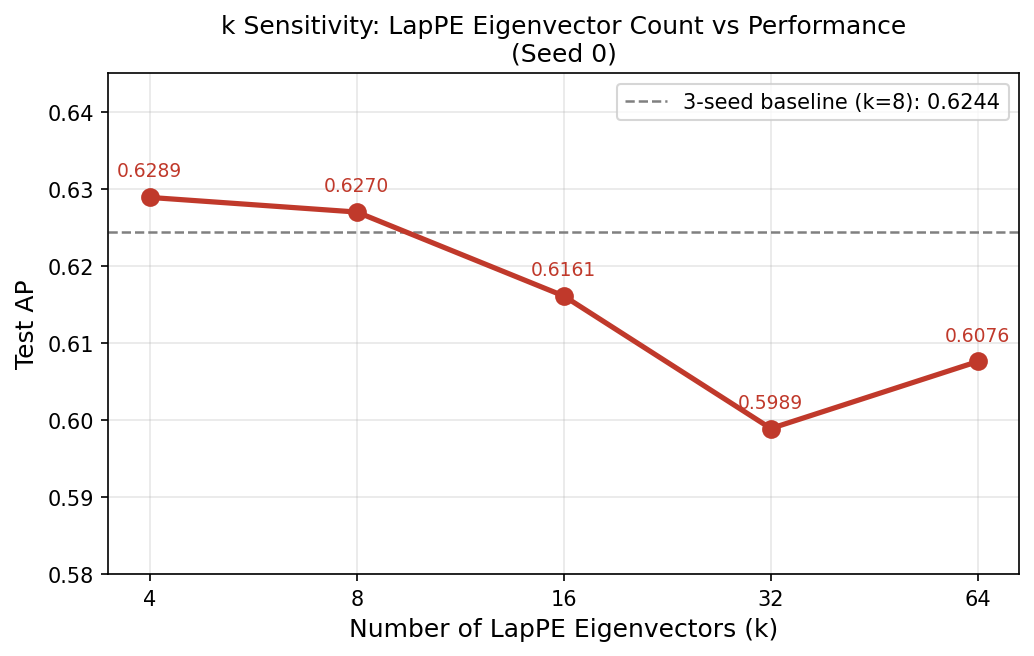
\includegraphics[width=0.65\linewidth]{k_sensitivity.png}
  \caption{Test AP vs.\ number of LapPE eigenvectors $k$ (seed 0). The dashed line indicates the 3-seed baseline at $k{=}8$ (AP\,=\,0.6244).}
  \label{fig:k_sens}
\end{figure}

\subsection{Effective Receptive Field Analysis}
\label{sec:erf}

To verify whether spectral mixing achieves genuine long-range information flow, we compute gradient-based Effective Receptive Field (ERF) scores \citep{luo2016understanding}. We evaluate both a single 89-node Peptides test graph and an aggregated sample of 50 test graphs to establish a statistically robust baseline. 

\begin{figure}[t]
  \centering
  \begin{minipage}{0.48\linewidth}
    \centering
    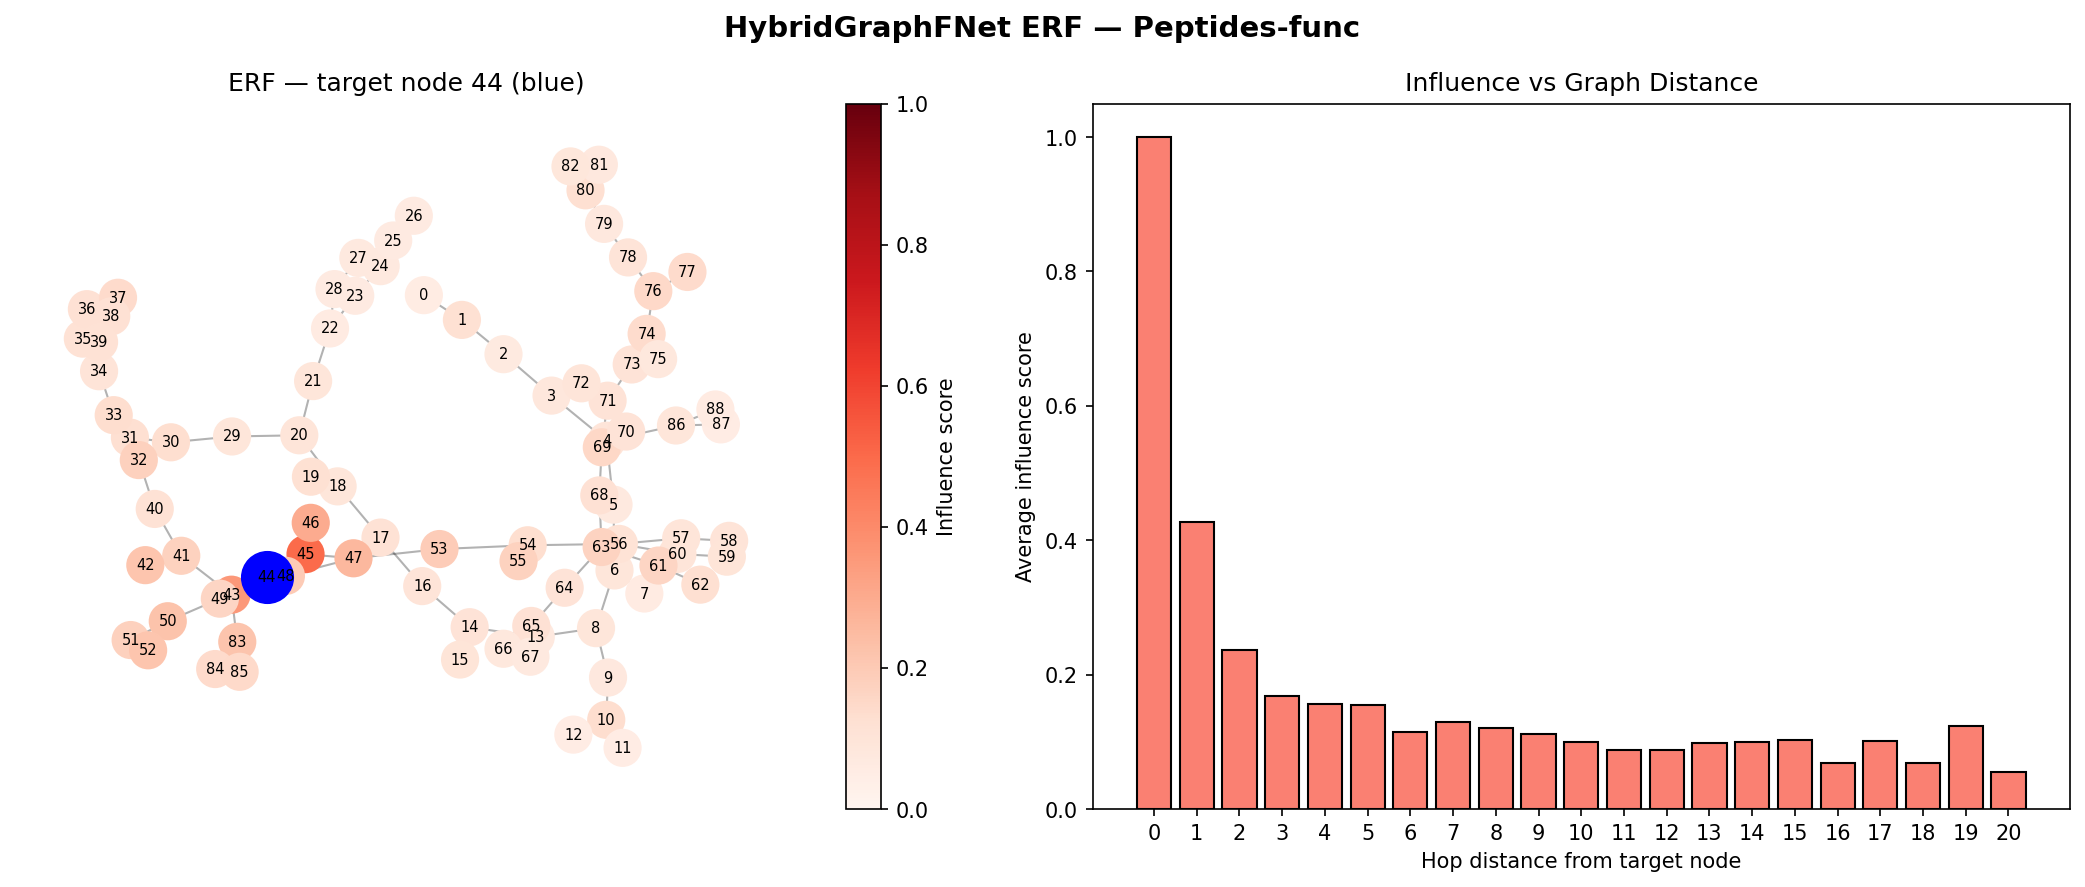
\includegraphics[width=\linewidth]{erf_func.png}
    \caption{ERF influence scores by hop distance on Peptides-func (single graph).}
    \label{fig:erf_func}
  \end{minipage}\hfill
  \begin{minipage}{0.48\linewidth}
    \centering
    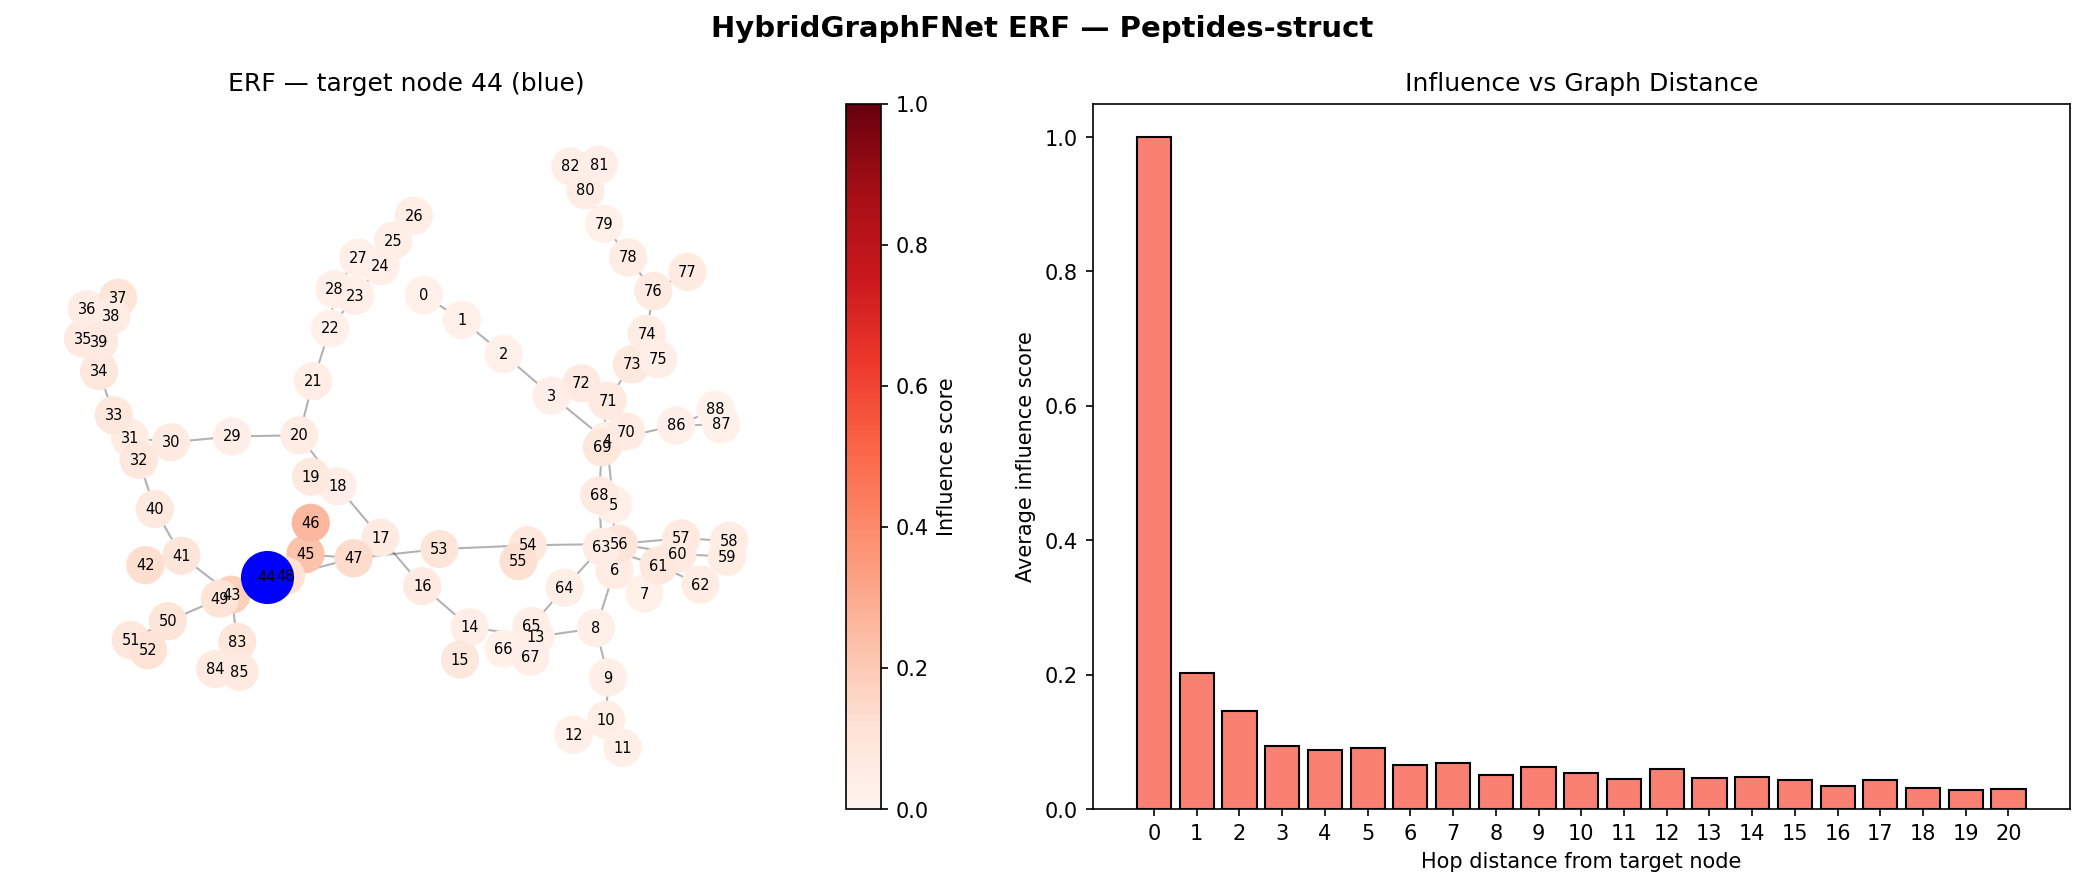
\includegraphics[width=\linewidth]{erf_struct.png}
    \caption{ERF influence scores by hop distance on Peptides-struct (single graph).}
    \label{fig:erf_struct}
  \end{minipage}
\end{figure}

\begin{table}[t]
\caption{Single-graph ERF influence by hop distance. A 4-layer GCN has zero influence beyond hop 4.}
\label{tab:erf_single}
\centering
\begin{tabular}{lccc}
\toprule
\textbf{Hop} & \textbf{Peptides-func} & \textbf{Peptides-struct} & \textbf{4-layer GCN} \\
\midrule
1  & 0.43 & 0.20 & ${\sim}1.0$ \\
5  & 0.15 & 0.07 & 0.00        \\
10 & 0.10 & 0.04 & 0.00        \\
20 & 0.06 & 0.03 & 0.00        \\
\bottomrule
\end{tabular}
\end{table}

\begin{table}[t]
\caption{Aggregated ERF influence across 50 randomly sampled test graphs (Mean $\pm$ SD).}
\label{tab:erf_aggregate}
\centering
\begin{tabular}{lccc}
\toprule
\textbf{Hop} & \textbf{Peptides-func} & \textbf{Peptides-struct} & \textbf{4-layer GCN} \\
\midrule
1  & $0.38 \pm 0.16$ & $0.26 \pm 0.12$ & ${\sim}1.0$ \\
5  & $0.17 \pm 0.06$ & $0.09 \pm 0.04$ & 0.00        \\
10 & $0.12 \pm 0.04$ & $0.06 \pm 0.02$ & 0.00        \\
20 & $0.07 \pm 0.03$ & $0.03 \pm 0.02$ & 0.00        \\
65 & $0.012 \pm 0.006$ & $0.005 \pm 0.003$ & 0.00        \\
\bottomrule
\end{tabular}
\end{table}

While a 4-layer GCN exhibits a hard receptive field cutoff at hop 4, GraphFNet maintains non-zero influence across the entire graph diameter (up to 65 hops in the aggregated dataset). This smooth, gradual influence decay confirms that the spectral operator establishes genuine long-range dependencies without self-attention.

Furthermore, the func model exhibits significantly stronger long-range influence ($0.07 \pm 0.03$ at hop 20) than the struct model ($0.03 \pm 0.02$). This aligns with chemical intuition: biological function relies heavily on global topology, whereas structural properties depend on local environments. The aggregated ERF data, obtained without any architectural modification between tasks, demonstrates that GraphFNet learns task-appropriate integration regimes, whether local or global, directly from the supervision signal.

Given recent questions regarding whether LRGB strictly requires long-range reasoning \citep{tonshoff2024where, bamberger2025measuring}, these mechanistic evaluations confirm that GraphFNet actively integrates distant node information regardless of the benchmark's inherent spatial demands.

\subsection{NeighborsMatch Diagnostic}
\label{sec:neighbors_match}

Long-range propagation is further evaluated on the Tree-NeighborsMatch diagnostic \citep{alon2021bottleneck}. The model must predict which half of a depth-$r$ binary tree contains a target leaf node, requiring exact $r$-hop signal propagation with no shortcut paths. This provides a strict, topology-bound test of long-range routing.

\begin{table}[t]
\caption{NeighborsMatch accuracy by tree depth $r$.}
\label{tab:nm}
\centering
\begin{tabular}{lcccc}
\toprule
\textbf{$r$} & \textbf{Nodes} & \textbf{GraphFNet} & \textbf{GCN (4-layer)} & \textbf{Random} \\
\midrule
2 & 7  & 100.0\% & 100.0\% & 50\% \\
3 & 15 & 100.0\% & 54.8\%  & 50\% \\
4 & 31 & 100.0\% & 52.0\%  & 50\% \\
5 & 63 & 50.2\%  & 50.2\%  & 50\% \\
\bottomrule
\end{tabular}
\end{table}

\begin{figure}[t]
  \centering
  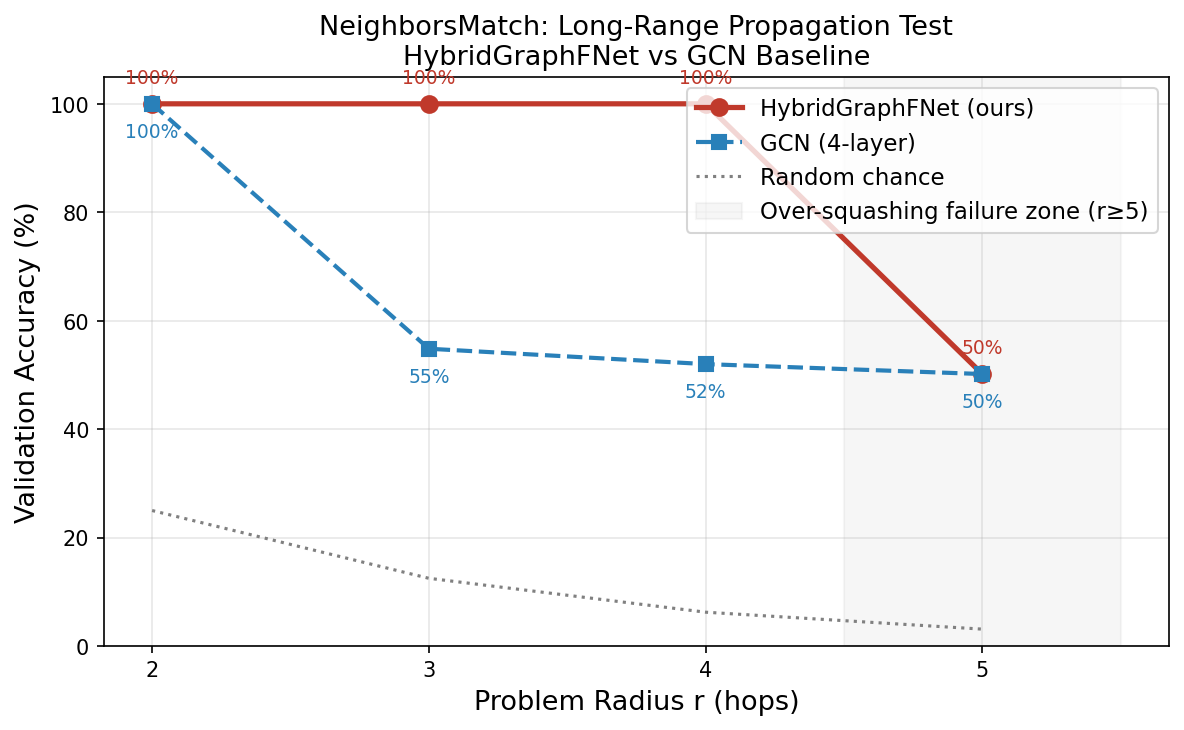
\includegraphics[width=0.65\linewidth]{neighbors_match_results.png}
  \caption{NeighborsMatch accuracy vs.\ tree depth $r$ for GraphFNet and a 4-layer GCN.}
  \label{fig:nm}
\end{figure}

GraphFNet achieves perfect 100\% accuracy for all problem radii up to $r{=}4$ ($r \in \{2, 3, 4\}$; Table~\ref{tab:nm}), successfully propagating signals where a depth-limited GCN collapses to near-random chance beginning at $r{=}3$ (54.8\% at $r{=}3$, 52.0\% at $r{=}4$). Although graph transformers can solve up to $r{=}6$ \citep{muller2024attending} by treating nodes as fully connected, effectively bypassing the tree topology, GraphFNet genuinely propagates information through the topology via its spectral pathway. Both models fail at $r{=}5$.

\paragraph{Mechanistic analysis of $r{=}5$ failure.}
To determine the root cause of the $r{=}5$ limitation, we analyze the algebraic connectivity ($\lambda_2$), gate profiles, and spectral resolution (see Table~\ref{tab:nm_mech} in Appendix~\ref{app:nm_details} for the complete breakdown). The value of $\lambda_2$ shrinks $19\times$ from $r{=}2$ (0.1835) to $r{=}5$ (0.0096), causing severe eigenvalue crowding near zero. However, increasing the basis to $k{=}32$ (covering over 50\% of the 63-node graph spectrum) fails to recover performance (yielding 53.2\% accuracy), confirming the breakdown is not a simple resolution limit.

Instead, the failure stems from the extreme structural symmetry of the depth-5 binary tree, which induces massive \textit{eigenvalue degeneracy}. As discussed in Section~\ref{sec:limitations}, when multiple eigenvectors share identical eigenvalues, the eigenspace exhibits continuous rotational ambiguity, rendering sign canonicalization insufficient. Crucially, the per-layer gate profiles at $r{=}5$ (mean $\approx 0.51$) remain indistinguishable from successful radii ($r{=}2$--$4$). The gating mechanism remains healthy and actively attempts to exploit the spectral pathway, but the spectral inputs themselves suffer from basis instability due to symmetry. This confirms that to scale attention-free spectral routing to highly symmetric graphs at large diameters, the architecture must integrate fully basis-invariant spectral encodings.

\subsection{Emergent Layer-Wise Specialization}
\label{sec:gate_analysis}

Analyzing the learned gating distributions on Peptides-func reveals an emergent \textbf{spectral-to-local routing progression} (where gates near 0 route through the global spectral pathway and gates near 1 favor local GCN aggregations; see Table~\ref{tab:gates} in Appendix~\ref{app:gate_stats} for complete per-layer statistics). The mean gate shifts monotonically from \textbf{0.356} in layer 0 (spectral-dominant) to \textbf{0.554} in layer 3 (local-dominant). Without explicit supervision, the model autonomously discovers an interpretable division of labor: early layers capture macro-scale molecular topology via spectral mixing, while later layers refine localized atom-level chemistry through GCN convolutions.

The high gate standard deviation at layer 0 (0.337) confirms significant per-node routing heterogeneity. Depending on their chemical context, individual atoms route near-entirely through spectral or local paths within the same layer. This validates the necessity of the per-node, per-feature gating mechanism; a scalar layer-wise gate would collapse this critical atom-level specificity. 

On the structurally uniform NeighborsMatch task, gates remain flat at ${\sim}0.50$ across all layers and radii. The contrast is highly informative: on Peptides, the model dynamically learns a task-appropriate layer-wise specialization; on NeighborsMatch, it correctly identifies that uniform mixing suffices. This depth-wise interpretability is a significant advantage over attention-based transformers (like GPS or SAN), which apply global attention uniformly across layers without structural incentive for specialization.

\subsection{Empirical Memory and Scalability Analysis}
\label{sec:vram_scaling}

To empirically validate the theoretical memory complexity of GraphFNet against standard dense-attention graph transformers, we conduct systematic VRAM scaling benchmarks on synthetic Erd\H{o}s-R\'enyi random graphs \citep{erdos1959random} across node counts from $N=200$ to $N=50,000$ (with hidden dimension $d=128$, 4 heads, on an NVIDIA GPU). Complete numerical tables for all scaling experiments are provided in Appendix~\ref{app:vram_tables}. We note that these comparisons are against \textit{standard dense self-attention}; profiling against efficient sub-quadratic attention methods (e.g., Exphormer \citep{shirzad2023exphormer}, NodeFormer \citep{wu2022nodeformer}) at HCP-comparable scales ($N=1{,}000$) is an important direction for future work that would require additional compute budget.

\begin{figure}[t]
  \centering
  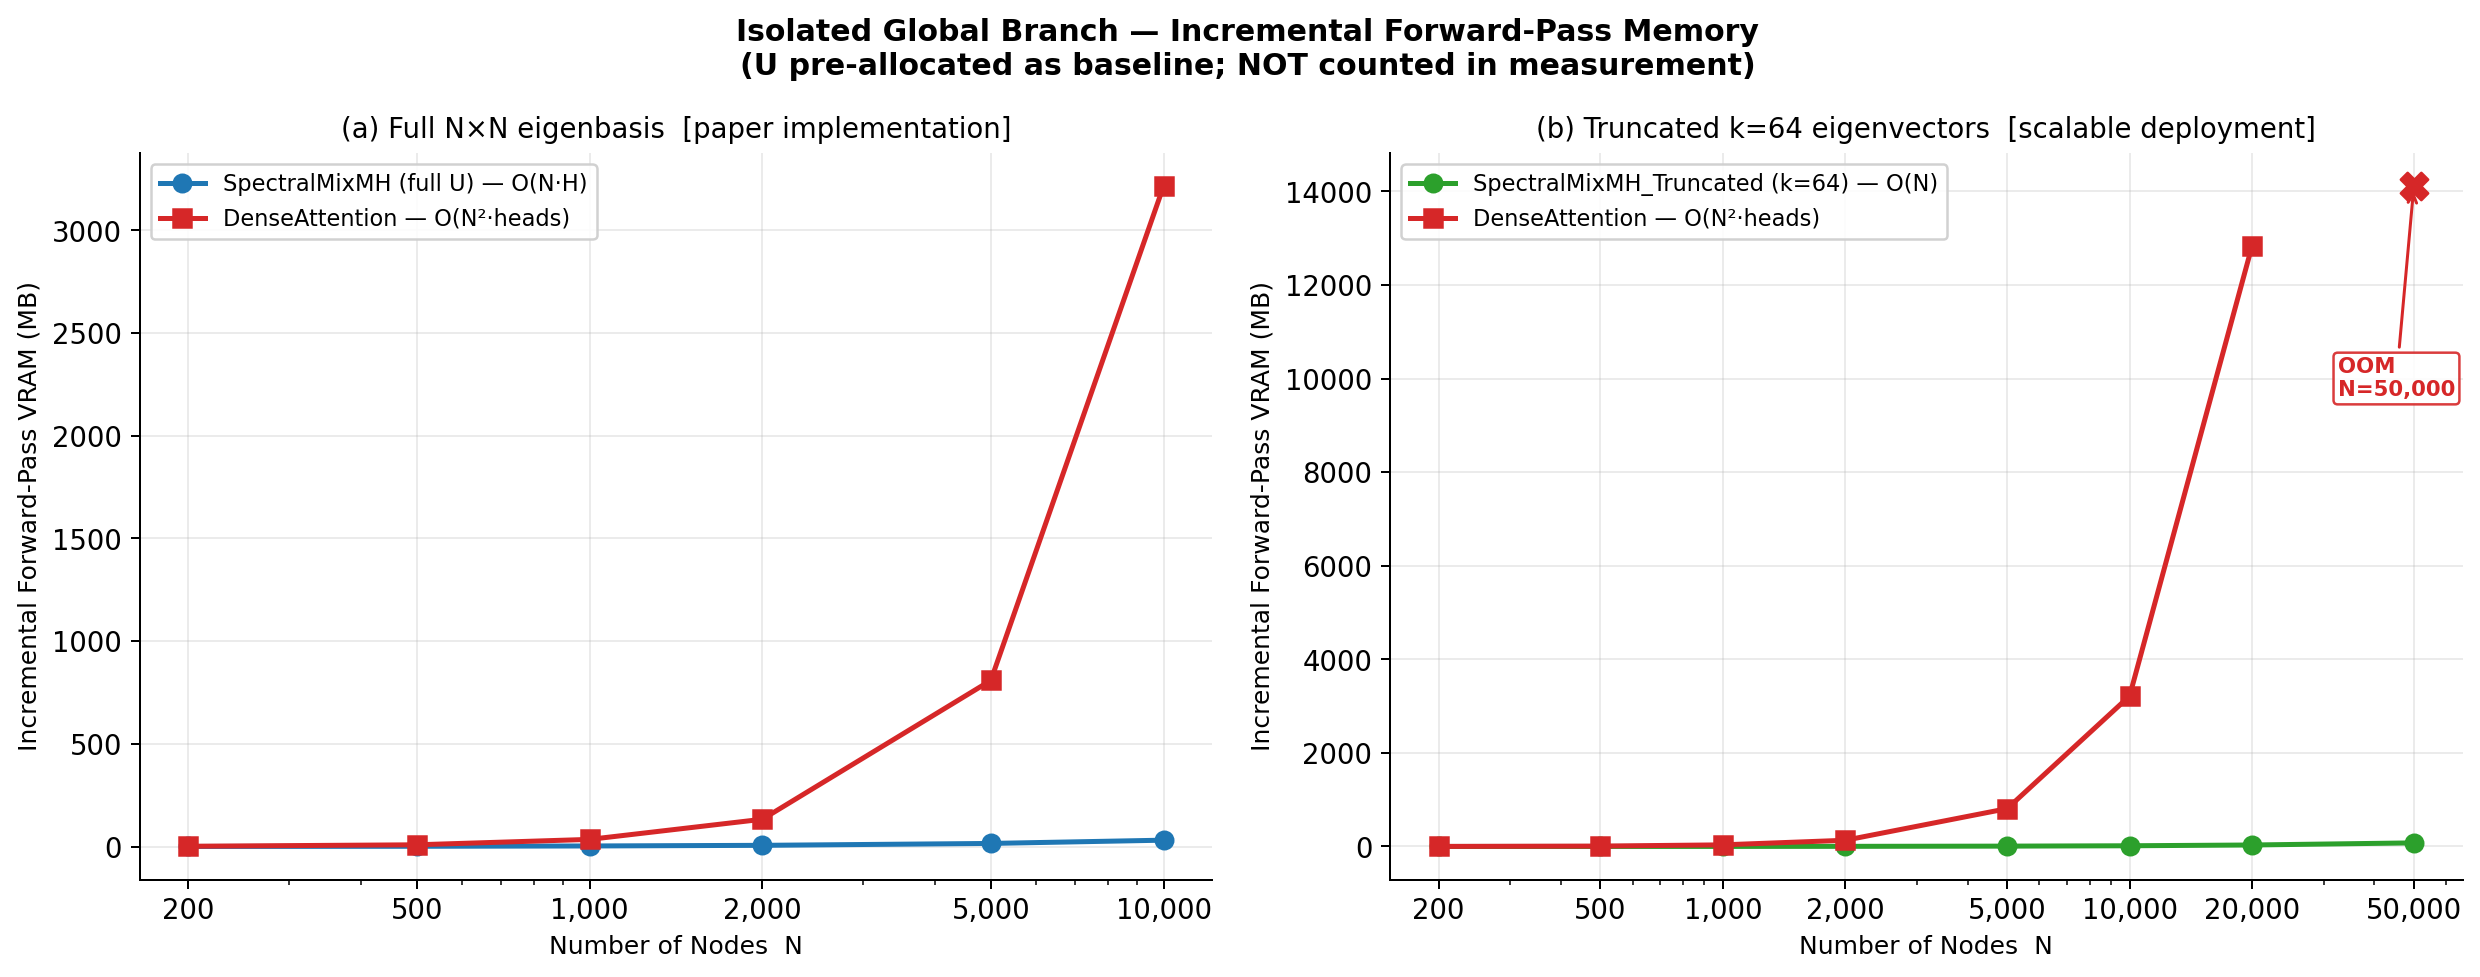
\includegraphics[width=\linewidth]{exp1_isolated_global_branch.png}
  \caption{Incremental forward-pass activation memory scaling for isolated global mixing operators across node counts $N$. (a) Full $N \times N$ eigenbasis ($U \in \mathbb{R}^{N \times N}$), showing $\mathcal{O}(N \cdot H)$ scaling for SpectralMix vs.\ quadratic $\mathcal{O}(N^2 \cdot H_{\text{heads}})$ scaling for dense self-attention. (b) Scalable deployment using truncated eigenbasis ($k=64$), maintaining linear scaling up to $N=50,000$ where self-attention fails with CUDA Out-Of-Memory (OOM).}
  \label{fig:exp1_vram}
\end{figure}

\paragraph{Isolated Global Branch Scaling.} Figure~\ref{fig:exp1_vram} (and Table~\ref{tab:vram_scaling} in Appendix~\ref{app:vram_tables}) confirms that the spectral mixing operator exhibits strict $\mathcal{O}(N \cdot H)$ activation memory scaling, whereas dense self-attention scales quadratically as $\mathcal{O}(N^2 \cdot H_{\text{heads}})$. At $N=10,000$, spectral mixing requires only 31.3~MB versus 3,215.6~MB for self-attention ($102.8\times$ reduction). When utilizing a truncated basis ($k=64$), spectral mixing remains strictly linear ($\mathcal{O}(N \cdot k \cdot H)$), executing at $N=50,000$ in 77.3~MB where dense self-attention encounters CUDA out-of-memory (OOM).

\begin{figure}[t]
  \centering
  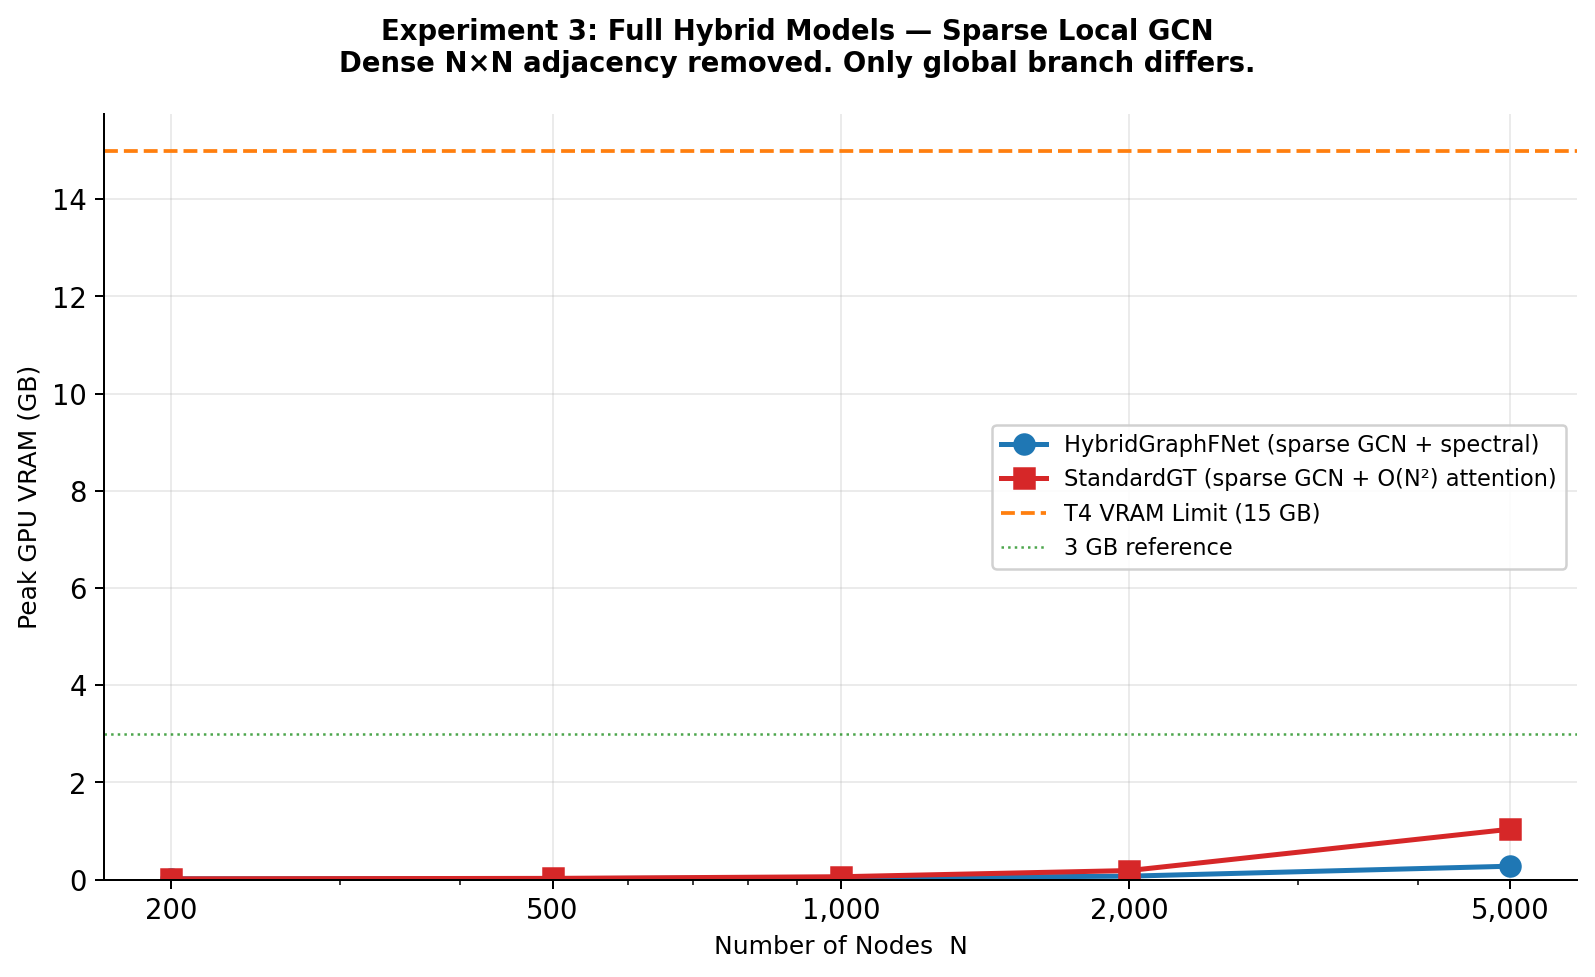
\includegraphics[width=0.65\linewidth]{exp3_full_sparse_models.png}
  \caption{Full 4-layer model peak GPU VRAM with sparse local GCN branch (\texttt{GCNConv} with native scalar edge gating). By eliminating the dense adjacency matrix confound, the global operator difference is cleanly isolated, demonstrating up to $3.78\times$ memory reduction before self-attention OOMs.}
  \label{fig:exp3_vram}
\end{figure}

\paragraph{Realistic Full-Model Deployment.} In Figure~\ref{fig:exp3_vram} (and Table~\ref{tab:full_sparse} in Appendix~\ref{app:vram_tables}), we evaluate complete 4-layer models where the local message-passing branch uses sparse \texttt{GCNConv} with scalar edge gating in both architectures, cleanly isolating the global operator. GraphFNet achieves up to $3.78\times$ memory savings at $N=5,000$ (0.274~GB vs.\ 1.036~GB), confirming real deployment advantages on commodity accelerators.

\begin{figure}[t]
  \centering
  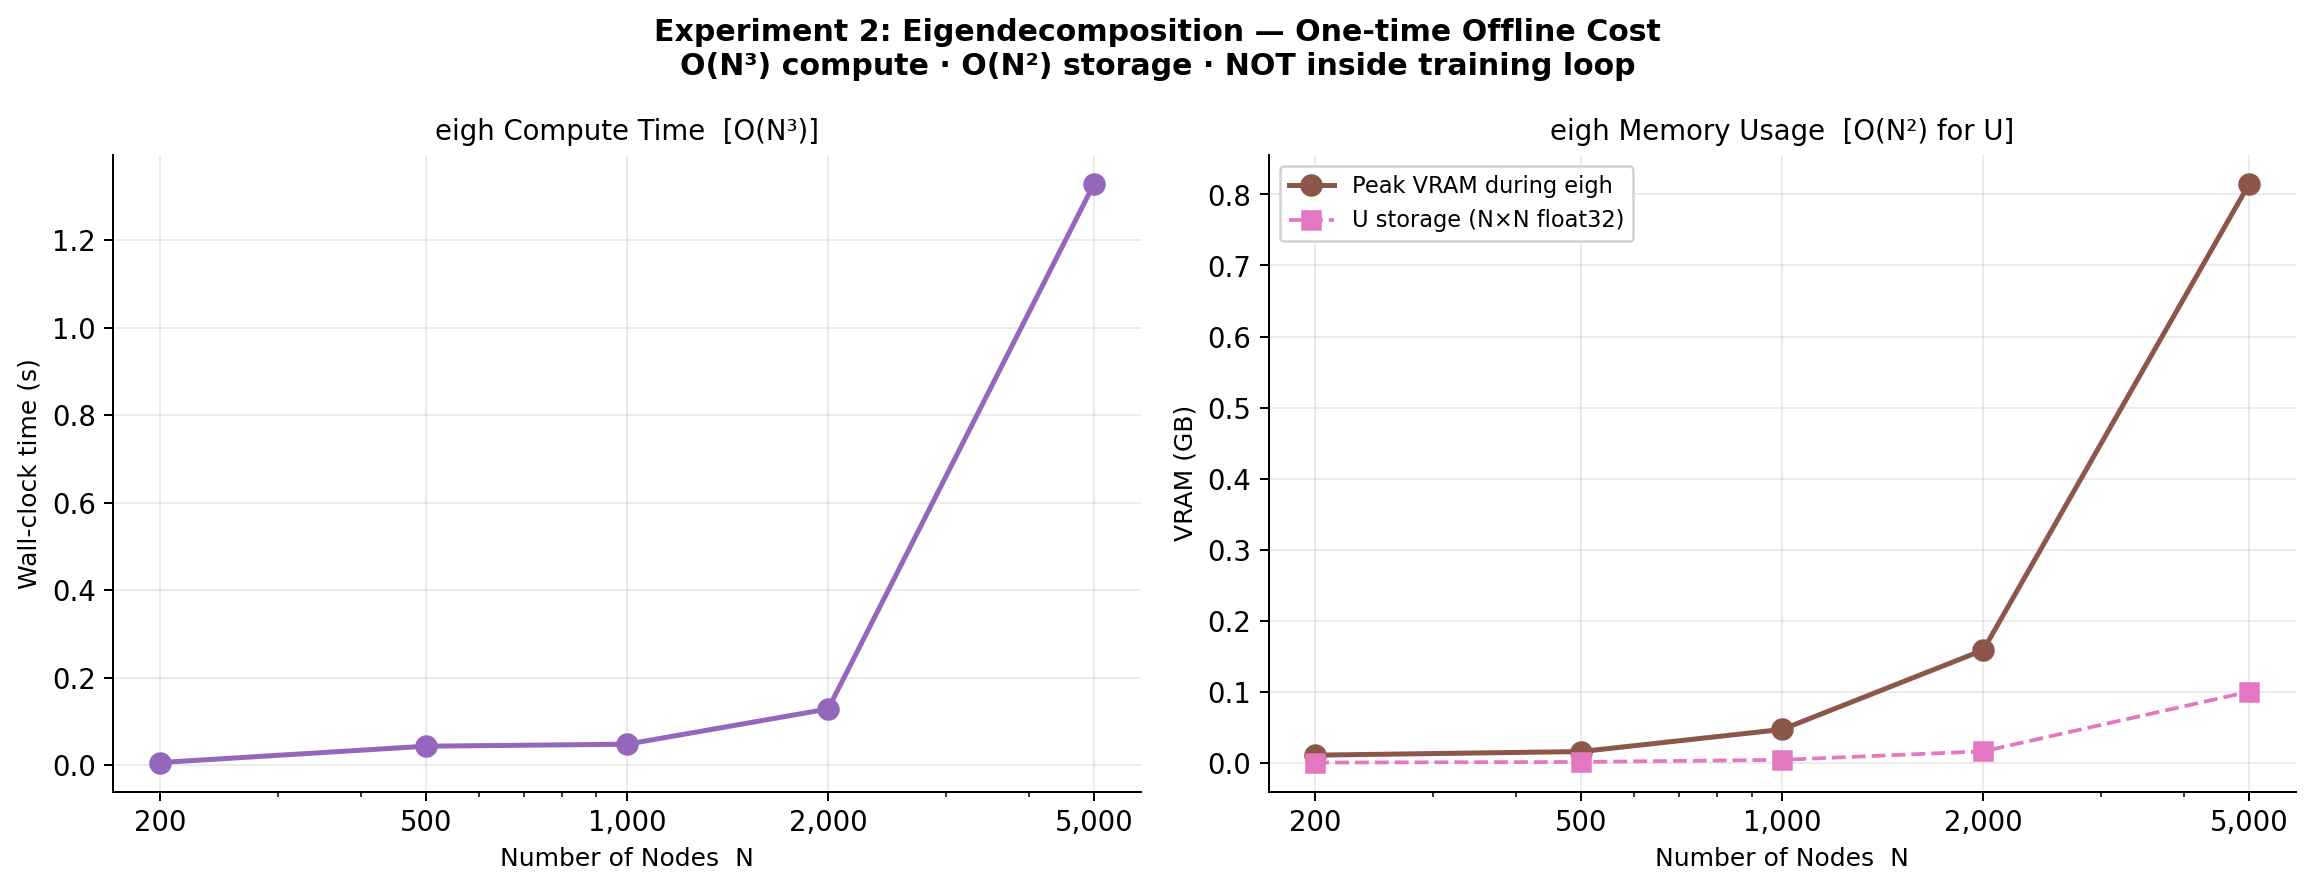
\includegraphics[width=\linewidth]{exp2_eigendecomp_cost.png}
  \caption{One-time offline Laplacian eigendecomposition cost (\texttt{torch.linalg.eigh}) across graph sizes $N$. (Left) Compute wall-clock time showing $\mathcal{O}(N^3)$ asymptotic scaling. (Right) Peak working VRAM during decomposition and basis tensor $U$ disk storage ($\mathcal{O}(N^2)$). Decoupling via offline caching eliminates this cost from the active training loop.}
  \label{fig:exp2_eigh}
\end{figure}

\paragraph{Disclosed Eigendecomposition Tradeoff.} Figure~\ref{fig:exp2_eigh} and Table~\ref{tab:eigh_cost} (Appendix~\ref{app:vram_tables}) transparently document the one-time offline eigendecomposition cost. For moderate-scale molecular graphs ($N \approx 150$), \texttt{eigh} takes $<0.05$~s per graph (0.006~s at $N=200$, 0.044~s at $N=500$), which is negligible relative to per-epoch training time. Because graph Laplacians are static, this basis is computed once offline and cached on disk at zero ongoing training cost. However, because \texttt{eigh} compute scales as $\mathcal{O}(N^3)$ (1.328~s at $N=5,000$), it represents a genuine precomputation constraint for massive graphs ($N \gtrsim 2{,}000$), as discussed in Section~\ref{sec:limitations}.

\subsection{Cross-Domain Transferability (BBBP)}

To evaluate whether the learned spectral-local gating paradigm transfers out-of-distribution to other molecular property prediction tasks, we evaluate GraphFNet on the Blood-Brain Barrier Penetration (BBBP) dataset \citep{wu2018moleculenet} under a strict Bemis-Murcko scaffold split across three random seeds. GraphFNet achieves a test ROC-AUC of \textbf{0.8686 $\pm$ 0.0203}, substantially outperforming standard unpretrained GCN baselines ($\sim$0.690 ROC-AUC) without chemistry-specific tuning. This confirms that the learned spectral-local representations generalize effectively across distinct molecular scaffolds.

\subsection{Summary of Findings}

The results collectively support six core empirical findings:
\begin{enumerate}[leftmargin=2em]
    \item \textbf{Attention-Free Spectral Mixing Efficiency:} Standard dense self-attention can be effectively replaced by learned spectral mixing over the Laplacian eigenbasis, achieving representation capability competitive with standard dense-attention graph transformers while using ${\sim}35$\% fewer parameters and reducing forward-pass activation memory by up to $3.78\times$ in full models ($102.8\times$ in isolated global branches; Section~\ref{sec:vram_scaling}). Eigendecomposition represents a disclosed one-time offline cost ($\mathcal{O}(N^3)$) that is decoupled from training via disk caching. We note that comparison against efficient sub-quadratic attention methods (e.g., Exphormer, NodeFormer, Specformer) remains an important open direction.
    \item \textbf{Critical Role of Per-Node Gating:} Per-node per-feature gating is co-equally essential to the spectral mixing operator. Ablation of either component results in an identical ${\sim}0.030$ AP collapse (Section~\ref{sec:ablation}), demonstrating that global routing and adaptive local-global integration are co-dependent.
    \item \textbf{Superiority and Scalability on Connectomics ($N=1,000$):} On dense irregular functional brain connectomes, GraphFNet establishes state-of-the-art accuracy on HCP-Gender (\textbf{81.17\% $\pm$ 1.90\%}, outperforming all baselines including BrainMAP at 78.92\%) and reaches \textbf{93.74\% $\pm$ 0.54\%} on 7-class HCP-Task (Table~\ref{tab:hcp_results}). Truncated spectral mixing ($k=64$) and \textbf{GatedPooling} enable seamless scaling under 2.53~GB VRAM with an $18.8\times$ caching speedup.
    \item \textbf{Inductive Bias Boundaries on Node-Level Segmentation:} On PascalVOC-SP superpixel graphs (Section~\ref{sec:pascalvoc_results}), GraphFNet outperforms standard message passing (0.1443 vs.\ 0.1268 GCN) with 39\% fewer parameters, but diagnoses a fundamental inductive bias boundary: while global spectral mixing is constructive for whole-graph pooling ($h_G = \text{GatedPooling}(H)$), it acts as low-pass spatial diffusion across 2D boundaries, delineating where static spectral routing excels versus where dynamic attention is uniquely advantaged.
    \item \textbf{Mechanistic Long-Range Signal Propagation:} Independent mechanistic probes confirm genuine long-range signal flow, with non-zero Effective Receptive Field influence maintained across graph diameters up to 65 hops (Section~\ref{sec:erf}) and 100\% accuracy on Tree-NeighborsMatch up to $r=4$ (where depth-limited message passing collapses beginning at $r=3$; Section~\ref{sec:neighbors_match}), circumventing message-passing over-squashing.
    \item \textbf{Emergent Routing Interpretability:} Layer-wise gate analysis reveals an autonomous spectral-to-local routing curriculum (Section~\ref{sec:gate_analysis}), capturing global topology in early layers before refining local chemistry in later layers. Out-of-distribution evaluation on BBBP (0.8686 ROC-AUC) confirms robust cross-domain scaffold transferability.
\end{enumerate}

%% ---------------------------------------------------------------
\section{Conclusion}
%% ---------------------------------------------------------------

In this work, we presented GraphFNet, a parameter-efficient, attention-free architecture that replaces the dynamic quadratic memory footprint of standard dense self-attention with static spectral mixing over the graph Laplacian eigenbasis, paired with local GCN aggregations through a novel per-node, per-feature gating mechanism.

Across molecular (LRGB Peptides), neuroimaging (NeuroGraph HCP, $N=1{,}000$), vision (PascalVOC-SP), and out-of-distribution (BBBP) benchmarks, our evaluations reveal a clear picture of when static spectral routing excels and where it encounters fundamental inductive bias boundaries. On graph-level tasks where global topology is decisive, spectral mixing matches or outperforms standard dense-attention transformers with substantially fewer parameters; on the large-scale HCP-Gender connectomics benchmark, GraphFNet achieves state-of-the-art accuracy. Conversely, on node-level superpixel segmentation, static spectral diffusion trades local boundary precision for holistic topology, delineating the complementary strengths of static spectral and dynamic attention routing.

Beyond predictive performance, we consider the architecture's most distinctive contribution to be the per-node, per-feature gating mechanism and the interpretability it affords. Ablation confirms that spectral mixing and per-node gating are co-dependent and co-equally critical. Mechanistic probing reveals that the model autonomously learns a spectral-to-local routing curriculum across layers, and ERF analysis confirms genuine long-range signal propagation across graph diameters of up to 65 hops. This emergent, interpretable division of labor between global and local pathways offers a qualitatively different form of transparency compared to attention-weight visualization.

We note two important caveats. First, our efficiency and performance comparisons are against standard dense-attention graph transformers; a growing family of efficient sub-quadratic attention methods (Exphormer, NodeFormer, Specformer) occupies a middle ground that we have not yet benchmarked against. Second, the $\mathcal{O}(N^3)$ eigendecomposition cost, while decoupled from training via offline caching, remains a genuine scalability constraint for very large graphs. Addressing both of these gaps is the primary focus of our ongoing work (Section~\ref{sec:limitations}).

%% ---------------------------------------------------------------
\section{Limitations and Future Work}
\label{sec:limitations}
%% ---------------------------------------------------------------

While GraphFNet establishes a strong foundation for attention-free graph learning, several limitations remain. First, the reliance on exact eigendecomposition incurs an $\mathcal{O}(N^3)$ computational cost, restricting the immediate applicability of the current implementation to medium-scale graphs unless offline caching or basis truncation is applied. Second, while the model achieves competitive results without exhaustive hyperparameter tuning, systematic optimization across a broader search space could yield further performance gains. Third, our empirical comparisons position GraphFNet against standard dense-attention graph transformers and established message-passing baselines; however, a growing family of efficient sub-quadratic attention methods---including Exphormer \citep{shirzad2023exphormer}, NodeFormer \citep{wu2022nodeformer}, and Specformer \citep{bo2023specformer}---retains content-dependent attention while reducing its quadratic cost. Direct comparison against this family would more precisely delineate GraphFNet's position in the efficiency-expressivity landscape and is an important direction for future evaluation. Finally, while we demonstrated transferability across molecular chemistry, cross-domain scaffold splits (BBBP), and large-scale functional connectomics, scaling to dynamic, time-evolving graphs or web-scale billion-edge networks remains to be explored in future studies.

A key theoretical limitation concerns the stability of the spectral basis in the presence of structural symmetry. While our largest-magnitude sign canonicalization effectively resolves simple sign ambiguity for distinct eigenvalues, it is unlikely to produce consistent eigenvector orientations across batches for degenerate eigenspaces. In cases where multiple eigenvectors share the same eigenvalue, a phenomenon observed in our NeighborsMatch experiments at $r=5$, the eigenspace exhibits full continuous rotational ambiguity. While our empirical results demonstrate that simple sign fixing is practically sufficient for organic molecular benchmarks like LRGB Peptides, a more mathematically rigorous approach would employ fully basis-invariant architectures, such as SignNet \citep{lim2023signnet}, to stabilize the spectral signal.

Future work will address computational constraints by transitioning from exact eigendecomposition to scalable, approximate spectral solvers, such as LOBPCG or randomized SVD, or by utilizing the offline spectral caching strategy demonstrated in our auxiliary experiments. Additionally, we plan to implement fully basis-invariant spectral encodings to resolve the limitations imposed by graph symmetry. Beyond architectural improvements, future evaluations will extend to diverse domains, including node-level prediction on heterophilous graphs and massive-scale network analysis, fully exploring the limits of spectral-local gating.


\bibliography{sample-base}
\bibliographystyle{tmlr}

\appendix

\section{Detailed $k$-Sensitivity Analysis}
\label{app:k_sensitivity}

To investigate the interaction between explicit Laplacian Positional Encodings (LapPE) and the implicit positional information provided by the SpectralMix operator, we systematically evaluate test AP on Peptides-func across eigenvector counts $k \in \{0, 4, 8, 16, 32, 64\}$ at seed 0 (illustrated in Figure~\ref{fig:k_sens}).

\begin{table}[h]
\centering
\caption{Test AP on Peptides-func across different LapPE eigenvector counts $k$ (evaluated at seed 0).}
\label{tab:k_sens_app}
\begin{tabular}{lcccccc}
\toprule
\textbf{Eigenvectors ($k$)} & \textbf{0 (No LapPE)} & \textbf{4} & \textbf{8 (Default)} & \textbf{16} & \textbf{32} & \textbf{64} \\
\midrule
\textbf{Test AP} & 0.6197 & 0.6289 & 0.6244 & 0.6120 & 0.5989 & 0.6076 \\
\bottomrule
\end{tabular}
\end{table}

While $k=4$ achieves a marginally higher single-seed result (0.6289), $k=8$ (0.6244 $\pm$ 0.0072 across 3 seeds) provides optimal cross-seed stability. Performance degrades monotonically for $k > 8$, experiencing a substantial drop at $k=32$ (0.5989) before partially recovering at $k=64$ (0.6076). This degradation highlights an interference effect: because the SpectralMix operator already applies the full Laplacian eigenbasis $U$ across all channels at every layer, injecting high-dimensional explicit eigenvectors into initial node features introduces redundant and conflicting coordinate signals. Consequently, explicit LapPE is best utilized as light augmentation ($k \le 8$) rather than a heavy positional mechanism in spectral-mixing architectures.

\section{NeighborsMatch Mechanistic Details and Spectral Gap}
\label{app:nm_details}

Table~\ref{tab:nm_mech} documents the algebraic connectivity ($\lambda_2$), classification accuracy, and layer-wise gate means across tree depths $r \in \{2, 3, 4, 5\}$ on the Tree-NeighborsMatch synthetic diagnostic \citep{alon2021bottleneck}.

\begin{table}[h]
\caption{Spectral gap ($\lambda_2$) and per-layer gate profiles across Tree-NeighborsMatch problem radii $r$.}
\label{tab:nm_mech}
\centering
\begin{tabular}{lccl}
\toprule
\textbf{$r$} & \textbf{$\lambda_2$} & \textbf{Accuracy} & \textbf{Gate means (layers 0--3)} \\
\midrule
2 & 0.1835 & 100\% & [0.51, 0.56, 0.55, 0.54] \\
3 & 0.0572 & 100\% & [0.48, 0.50, 0.51, 0.49] \\
4 & 0.0222 & 100\% & [0.52, 0.52, 0.46, 0.46] \\
5 & 0.0096 & 50.2\%  & [0.50, 0.51, 0.52, 0.51] \\
\bottomrule
\end{tabular}
\end{table}

As the problem depth increases from $r=2$ to $r=5$, the algebraic connectivity $\lambda_2$ decreases by a factor of 19, crowding non-zero eigenvalues near the origin. Increasing the basis capacity to $k=32$ (spanning more than half of the 63-node tree spectrum) yields only 53.2\% accuracy, confirming that the $r=5$ bottleneck is driven by eigenvalue degeneracy resulting from the high automorphic symmetry of complete binary trees rather than insufficient spectral resolution.

\section{Per-Layer Gate Statistics on Peptides-func}
\label{app:gate_stats}

Table~\ref{tab:gates} provides the complete empirical distribution of learned gating values across network layers on the Peptides-func test set.

\begin{table}[h]
\caption{Per-layer gate statistics on the Peptides-func test set.}
\label{tab:gates}
\centering
\begin{tabular}{lccc}
\toprule
\textbf{Layer} & \textbf{Mean Gate} & \textbf{Std} & \textbf{Dominant Character} \\
\midrule
0 & 0.356 & 0.337 & Spectral-dominant \\
1 & 0.341 & 0.191 & Spectral-dominant \\
2 & 0.417 & 0.154 & Transitioning     \\
3 & 0.554 & 0.195 & Local-dominant    \\
\bottomrule
\end{tabular}
\end{table}

The gating distribution demonstrates a consistent transition from global spectral processing in layers 0--1 ($\mu \approx 0.34$--$0.36$) to localized message passing in layer 3 ($\mu = 0.554$). The high variance in layer 0 ($\sigma = 0.337$) underscores that individual atom representations adaptively utilize distinct routing mixtures according to their local chemical environment.

\section{Complete Memory Scaling and Eigendecomposition Tables}
\label{app:vram_tables}

This section provides the full numerical scaling data corresponding to Section~\ref{sec:vram_scaling} on synthetic Erd\H{o}s-R\'enyi random graphs \citep{erdos1959random}.

\begin{table}[!htbp]
\caption{Incremental forward-pass activation memory scaling for isolated global mixing operators: SpectralMix (full $U \in \mathbb{R}^{N \times N}$ and truncated $k=64$) vs.\ dense Multi-Head Self-Attention on an NVIDIA GPU (hidden dimension $d=128$, 4 heads).}
\label{tab:vram_scaling}
\centering
\begin{tabular}{rcccc}
\toprule
\textbf{Nodes ($N$)} & \textbf{SpectralFull} & \textbf{SpectralTrunc ($k{=}64$)} & \textbf{DenseAttn} & \textbf{Ratio} \\
\midrule
200    & 0.6~MB  & 0.4~MB  & 1.6~MB      & $2.6\times$ \\
500    & 1.5~MB  & 0.9~MB  & 8.8~MB      & $5.7\times$ \\
1,000  & 3.1~MB  & 1.6~MB  & 35.1~MB     & $11.4\times$ \\
2,000  & 6.2~MB  & 3.2~MB  & 133.1~MB    & $21.6\times$ \\
5,000  & 15.4~MB & 7.8~MB  & 808.8~MB    & $52.5\times$ \\
10,000 & 31.3~MB & 15.5~MB & 3,215.6~MB  & $102.8\times$ \\
20,000 & --      & 32.0~MB & 12,832.5~MB & $401.5\times$ \\
50,000 & --      & 77.3~MB & \textbf{CUDA OOM} & -- \\
\bottomrule
\end{tabular}
\end{table}

\begin{table}[!htbp]
\caption{Full 4-layer model peak forward VRAM where the local branch uses sparse message passing (\texttt{GCNConv} with native scalar edge gating) in both backbones, isolating the global operator in a realistic deployment setting.}
\label{tab:full_sparse}
\centering
\begin{tabular}{rccc}
\toprule
\textbf{Nodes ($N$)} & \textbf{GraphFNet} & \textbf{Standard Graph Transformer} & \textbf{Ratio} \\
\midrule
200   & 0.013~GB & 0.014~GB & $1.01\times$ \\
500   & 0.019~GB & 0.023~GB & $1.23\times$ \\
1,000 & 0.032~GB & 0.057~GB & $1.77\times$ \\
2,000 & 0.069~GB & 0.184~GB & $2.69\times$ \\
5,000 & 0.274~GB & 1.036~GB & $\mathbf{3.78\times}$ \\
\bottomrule
\end{tabular}

\vspace{1.5em}

\caption{One-time offline Laplacian eigendecomposition cost across node counts $N$ with kernel warmup and multi-run median timing. At Peptides scale ($N \approx 150$), precomputation is fast ($<0.05$~s/graph). Decoupled from training via offline caching, this cost is disclosed as a genuine $\mathcal{O}(N^3)$ computational constraint for massive graphs ($N \ge 2{,}000$).}
\label{tab:eigh_cost}
\centering
\begin{tabular}{rccc}
\toprule
\textbf{Nodes ($N$)} & \textbf{\texttt{eigh} Time (s)} & \textbf{Peak VRAM (GB)} & \textbf{$U$ Storage (GB)} \\
\midrule
200   & 0.006~s & 0.1111~GB & 0.0002~GB \\
500   & 0.044~s & 0.1153~GB & 0.0010~GB \\
1,000 & 0.048~s & 0.1437~GB & 0.0040~GB \\
2,000 & 0.129~s & 0.2425~GB & 0.0160~GB \\
5,000 & 1.328~s & 0.9156~GB & 0.1000~GB \\
\bottomrule
\end{tabular}
\end{table}

\end{document}